%%%%%%%%%%%%%%%%%%%%%%%%%%%%%%%%%%%%%%%%%%%%%%%%%%%%%%%%%%%%%%%%%%%
%%% Documento LaTeX 																						%%%
%%%%%%%%%%%%%%%%%%%%%%%%%%%%%%%%%%%%%%%%%%%%%%%%%%%%%%%%%%%%%%%%%%%
% Título:		Introducción
% Autor:  	Ignacio Moreno Doblas
% Fecha:  	2014-02-01, actualizado 2019-11-11
% Versión:	0.5.0
%%%%%%%%%%%%%%%%%%%%%%%%%%%%%%%%%%%%%%%%%%%%%%%%%%%%%%%%%%%%%%%%%%%
% !TEX root = A0.TFG.tex

\chapterbegin{Estado del arte}
\minitoc

\todo[inline, size=\tiny]{Citar las referencias en la bibliografía de las que he obtenido la información del estado del arte}

\section{Cognición}
\label{sec:estadoArte:cognicion}

Uno de los factores que separa a los seres humanos del resto de animales es su mayor desarrollo cognitivo. La cognición es la capacidad para captar, asimilar, procesar y utilizar información obtenida del entorno. Bajo este nombre se incluyen diversos procesos cognitivos como: el aprendizaje, la memoria, la toma de decisiones, la comprensión y el razonamiento.

Los primeros estudios sobre la cognición, desarrollados por Aristóteles, datan del siglo IV A.C. Aristóteles estudió el funcionamiento interno de la mente humana centrándose en la memoria y la percepción. Siempre trató de basar sus estudios en técnicas puramente empíricas mediante la experimentación y la observación. \cite{EA_cog_aristoteles}

No fue hasta el siglo XV durante la Ilustración, que se retomaron los estudios sobre la mente y su funcionamiento. Y más significativamente, durante los siglos XIX y XX.

Durante la segunda mitad del siglo XIX, el auge y desarrollo de la psicología y especialmente de la psicología experimental, impulsó la investigación en el campo cognitivo. El filósofo y psicólogo alemán Wilhelm Wundt (1832-1920) desarrolló el concepto de introspección, una técnica consistente en el autoanálisis de los sentimientos de la persona, exponiéndolos de la forma más objetiva posible. \cite{EA_cog_wundt} La introspección sentó las bases para el desarrollo de las técnicas posteriores, aunque debido a ser puramente subjetiva los psicólogos posteriores intentarán no depender de ella.

Hermann Ebbinghaus (1850-1909), otro psicólogo alemán, dedicó su carrera a la investigación de la memoria. Desarrolló un experimento con el que probar la capacidad de aprendizaje de nueva información, así como la pérdida de ella mediante el olvido. Debido a que el experimento debía evitar la intervención de cualquier conocimiento previo, Ebbinghaus creó hasta 2300 sílabas inexistentes y sin sentido para evitar ser asociadas con palabras reales. La prueba consistía en memorizar en orden aleatorio la mayor cantidad de dichas sílabas y recitarlas posteriormente. El experimento concluyó que el cerebro humano siempre intenta relacionar la nueva información con algún conocimiento anterior, y cuanto mayor es la relación encontrada mejor es la retención en la memoria de la nueva información. \cite{EA_cog_ebbinghaus}

Los estudios de Ebbinghaus le permitieron definir el efecto de posición serial (figura \ref{fig:EA_posicionSerial}): a la hora de memorizar y recitar una lista de elementos, la posición en la lista que ocupan los elementos tiene efecto en la capacidad para memorizarlos. El cerebro humano es capaz de retener mejor la información al principio de una lista (efecto de primacía) así como al final de esta (efecto de recencia), sin embargo, los elementos centrales son que mayor esfuerzo requieren para ser memorizados.



\begin{figure}
  \centering
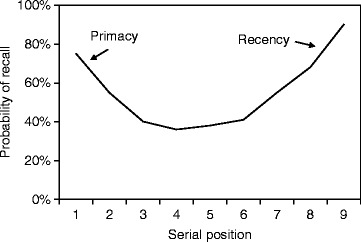
\includegraphics[width=0.5\textwidth]{03.EstudioProblema/01.EstadoArte/00.Figuras/01.efecto_serial.jpg}
    \caption{Gráfica que representa la curva creada por el efecto se posición serial. \cite{EA_img_efectoPosicionSerial}}
    \label{fig:EA_posicionSerial}
\end{figure}


La cognición y las habilidades y procesos cognitivos van evolucionando a lo largo de la vida de las personas.

Jean Piaget fue un psicólogo suizo que investigó el desarrollo cognitivo en el ser humano durante los primeros años de vida. Tras sus investigaciones concluyó que el desarrollo de los procesos cognitivos puede ser clasificado por etapas de crecimiento: \cite{EA_cog_piaget}

\begin{itemize}
	\item{Etapa sensomotora (0-2 años): Existe inteligencia, pero el conocimiento se basa únicamente en las experiencias. Se desarrollan las capacidades básicas de habla y de comprensión del espacio y el tiempo.}

	\item{Etapa preoperacional (2-7 años): Se desarrolla la memoria y la imaginación. Predomina la resolución intuitiva de problemas y el pensamiento egocéntrico.}

	\item{Etapa operacional concreta (7-12 años): El pensamiento deja de ser egocéntrico y pasa a ser más sistemático y lógico. Se entienden conceptos complejos espaciales y la persona puede utilizar un proceso de pensamiento reversible.}

	\item{Etapa operacional formal (+12 años): La capacidad de pensamiento se vuelve mucho más flexible, con la posibilidad de comprender conceptos abstractos y formular hipótesis para resolver problemas complejos.}

\end{itemize}

Durante la vida de una persona estas capacidades cognitivas adquiridas durante la infancia pueden resultar dañadas, degradadas o incluso perdidas completamente, dificultando o impidiendo a la persona realizar procesos como la toma de decisiones, aprendizaje o la evaluación crítica, así como llevando a la pérdida de memoria, capacidad de expresión o velocidad de procesado de información. \cite{EA_cog_deterioro}

La pérdida de estas capacidades puede estar causada o ser la causa de alguna enfermedad, por ejemplo: el deterioro cognitivo leve, en la que el paciente no puede llevar a cabo algunos procesos cognitivos de la forma esperada pero no afecta en gran medida a su vida diaria.

Trastornos más graves como la enfermedad de Alzheimer pueden llevar a peores consecuencias como la pérdida completa de la memoria inmediata, degradación en las capacidades cognitivas superiores y dificultad en la comunicación movimiento y resolución de problemas abstractos sencillos. \cite{EA_cog_alzheimer}

Incluso en personas sanas, las capacidades cognitivas van disminuyendo con el tiempo, especialmente durante la vejez. Esta degradación es esperada y no conlleva grandes problemas a la vida diaria de las personas. Para frenar y limitar lo máximo posible está degeneración es imprescindible mantener un alto nivel de actividad cognitiva. Este es el objetivo del entrenamiento cognitivo.




\section{Entrenamiento cognitivo}

El entrenamiento cognitivo, también llamado brain training, engloba al conjunto de actividades diseñadas para mantener o mejorar las capacidades cognitivas propias de una persona.

Estas actividades se basan en la neuroplasticidad humana, que significa que el cerebro es capaz de desarrollarse y transformarse en base a las experiencias vividas. Esto implica que el cerebro puede ser entrenado para fomentar el desarrollo de ciertas áreas de este involucradas con los procesos cognitivos. \cite{EA_ent_plasticidad}

Las áreas objetivo de entrenamientos más usuales son aquellas con mayor relación con actividades diarias y por tanto pueden conllevar una mejora notable de las habilidades. La capacidad de memorizar, mantener la atención y la resolución de problemas son los principales procesos que entrenar.

El entrenamiento cognitivo se centra en grupos de personas con carencias cognitivas como aquellas con enfermedades neurodegenerativas como la demencia o el Alzheimer. Aunque todas las personas pueden beneficiarse del entrenamiento, especialmente personas de edad avanzada que con el paso de los años han visto mermadas sus capacidades habituales en memorización, velocidad de procesamiento, razonamiento o psicomotricidad.

El resultado del brain training puede ser muy diverso entre las personas debido a que cada una tiene un rendimiento máximo en cada habilidad. Una vez que el individuo alcanza su estado óptimo en dicha habilidad, le supondrá un esfuerzo mucho mayor continuar mejorando.

Además, hay que tener en cuenta que incluso cuando el entrenamiento mejora las capacidades cognitivas básicas, estas mejoras pueden no trasladarse a acciones más complejas, a pesar de que dichas acciones sean combinaciones de habilidades sencillas.

A día de hoy, la verdadera efectividad del entrenamiento cognitivo está en duda. Los estudios más recientes demuestran que los grandes efectos de antienvejecimiento y prevención de la enfermedad de Alzheimer son falsos y exagerados por las técnicas de marketing. Si bien el entrenamiento tiene un efecto positivo en las habilidades cognitivas, existen otros factores con mayor importancia, como la genética de cada persona. \cite{EA_ent_efectividad}


\section{Ejercicios de Brain Training}
\label{sec:estadoArte:ejerciciosBrainTraining}

Los ejercicios de entrenamiento cognitivo se pueden presentar en multitud de formatos, comenzando por el formato físico en papel. Los cuadernos de ejercicios han sido el medio clásico de realizar entrenamientos cognitivos. Permiten la estimulación mediante el uso de una herramienta conocida, como es el lápiz y papel, a la vez que presenta ejercicios muy variados: memoria, razonamiento, resolución de problemas o comprensión lectora, adaptados a cualquier nivel, desde niños pequeños hasta personas mayores o enfermos. Su sencillez permite que sean fáciles de diseñar, fabricar y distribuir.

\subsection{Cuadernos de ejercicios}

Los cuadernos de estimulación cognitiva de Esteve (figura \ref{fig:EA_cuadernoEsteve}) y Rubio (figura \ref{fig:EA_cuardernoRubio}) son las más populares en España, están enfocados a personas con algún tipo de deterioro cognitivo (leve, moderado o grave) y su estructura de niveles permite una fácil clasificación y progreso en los ejercicios. \cite{EA_ent_esteve}






\begin{figure}[H]
\centering
\begin{minipage}{.5\textwidth}
  \centering
  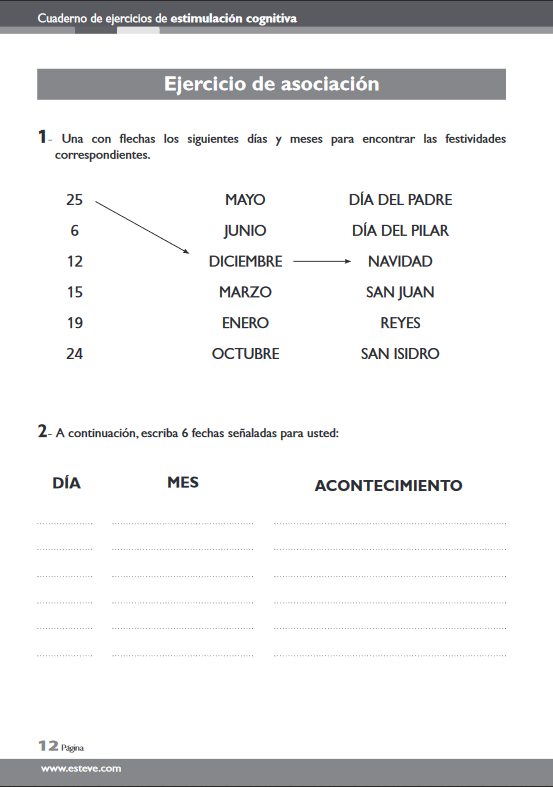
\includegraphics[width=.7\linewidth]{03.EstudioProblema/01.EstadoArte/00.Figuras/02.cuaderno_esteve.png}
  \captionof{figure}{Cuaderno Esteve. \cite{EA_img_cuadernoEsteve}}
  \label{fig:EA_cuadernoEsteve}
\end{minipage}%
\begin{minipage}{.5\textwidth}
  \centering
  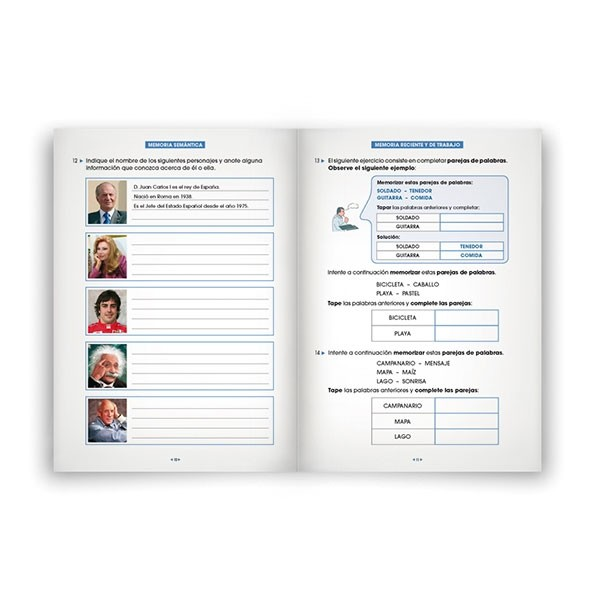
\includegraphics[width=.9\linewidth]{03.EstudioProblema/01.EstadoArte/00.Figuras/03.cuaderno_rubio.jpg}
  \captionof{figure}{Cuaderno Rubio. \cite{EA_img_cuardernoRubio}}
  \label{fig:EA_cuardernoRubio}
\end{minipage}
\end{figure}



\subsection{Juegos grupales}

En ocasiones donde varias personas que vayan a realizar un entrenamiento cognitivo se encuentren juntas, como residencias o centros de día para mayores, se pueden realizar juegos grupales. Estos juegos permiten no solo la mejora de las capacidades cognitivas por los ejercicios si no que también impulsan las relaciones interpersonales y fomentan la creación de un ambiente amigable y alegre durante la sesión de entrenamiento. \cite{EA_ent_grupos}

Estos juegos están diseñados para ser llevados a cabo en grupos: ya sea de forma simétrica, donde cada participante tiene un rol idéntico, o no, en los que una o varias personas ocupan un papel principal en la acción y el resto los complementa con diferentes acciones.

Existen multitud de juegos de este tipo, algunos de ellos son:

\begin{itemize}
	\item{Juego del abanico: Una persona toma el papel principal y debe transmitir al resto una emoción que elija mediante el uso únicamente de movimientos del abanico.}

	\item{Juego de expresiones: Una persona intenta expresar un sentimiento con expresiones faciales y el resto tendrá que adivinarlo.}

	\item{Juego de los nombres: Todos los participantes forman un círculo y por orden deberán decir su nombre y pasar una pelota al siguiente participante. Tras una vuelta completa, cada persona tendrá que decir algo que le guste y lanzar la pelota a cualquier participante diciendo su nombre. Véase figura \ref{fig:EA_juegosAncianos}}

\end{itemize}


\begin{figure}
  \centering
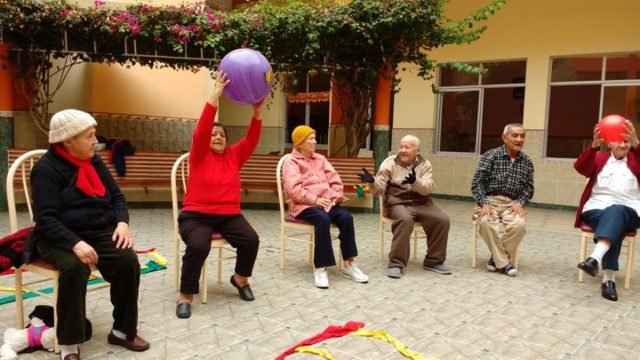
\includegraphics[width=0.8\textwidth]{03.EstudioProblema/01.EstadoArte/00.Figuras/04.juegos_ancianos.jpg}
    \caption{Juego de grupo con pelota. \cite{EA_img_juegoGrupoPelota}}
    \label{fig:EA_juegosAncianos}
\end{figure}

\subsection{Juegos y plataformas online}

Con la proliferación de las nuevas tecnologías en la vida diaria de las personas, los ejercicios de estimulación se han adaptado para sacar todo el provecho que estas tecnologías ofrecen. Los ejercicios clásicos en papel que ofrecen los cuadernos son fácilmente adaptables a un entorno digital mediante el uso de aplicaciones, juegos y páginas web, que son presentados al usuario a través de un ordenador o de un dispositivo móvil como una Tablet.

Este formato es capaz de enriquecer los ejercicios ya que añade la posibilidad de personalizar cada ejercicio para el nivel y las características del usuario, así como usar animaciones, sonidos y nuevos métodos de interacción: pantalla táctil, movimiento del propio dispositivo, reconocimiento de voz, etc.

Estas plataformas online permiten un monitoreo constante de un profesional sin necesidad de estar físicamente presente con el paciente lo que puede aumentar su utilidad y eficacia frente a los cuadernos tradicionales.

\subsubsection{Lumosity}

Lumosity es una aplicación que reúne una serie de juegos muy llamativos para entrenar la mente de manera amena y dinámica. Se categorizan según la habilidad cognitiva que tratan: velocidad de procesamiento, memoria, atención, flexibilidad mental y resolución de problemas. En la figura \ref{fig:EA_lumosity} se pueden ver varios de estas categorías y sus juegos. \cite{EA_ent_lumosity}

\begin{figure}
  \centering
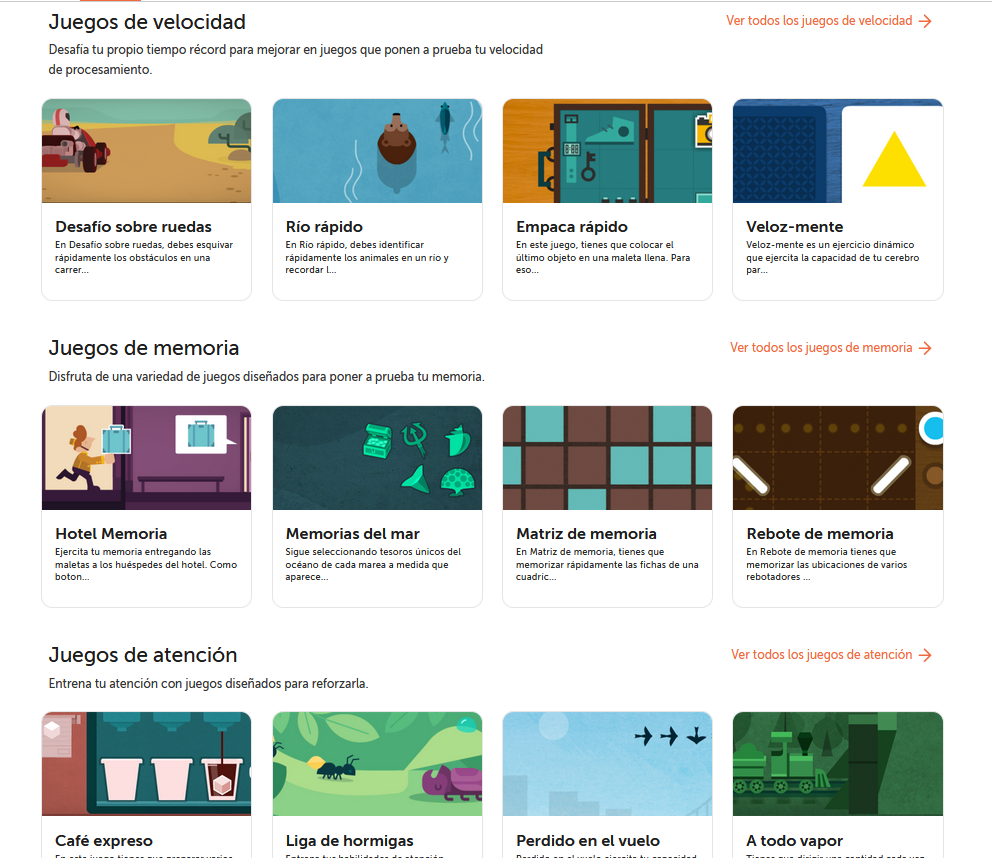
\includegraphics[width=0.5\textwidth]{03.EstudioProblema/01.EstadoArte/00.Figuras/05.lumosity.png}
    \caption{Algunos de los juegos disponibles en Lumosity.}
    \label{fig:EA_lumosity}
\end{figure}


\subsubsection{NeuronUp}

NeuronUp es una plataforma multidispositivo (figura \ref{fig:EA_neuronUp}) enfocada al uso de profesionales para monitorizar los entrenamientos de sus pacientes. Los juegos son más simples que los de Lumosity, pero ofrece una conexión directa y constante con los profesionales, que es importante para llevar un correcto entrenamiento. \cite{EA_ent_neuronup}

\begin{figure}
  \centering
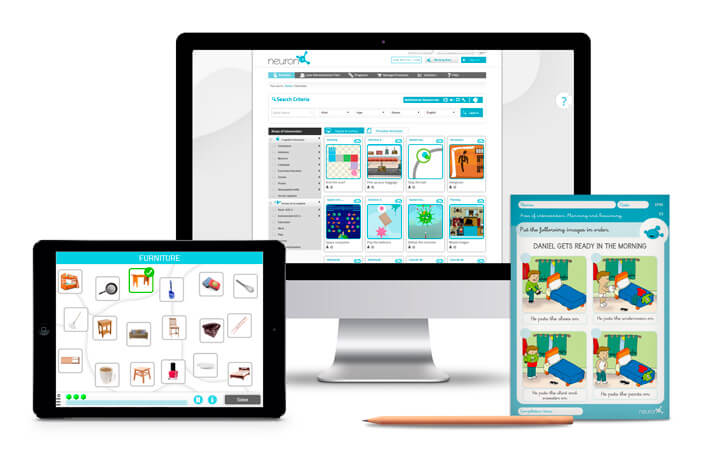
\includegraphics[width=0.5\textwidth]{03.EstudioProblema/01.EstadoArte/00.Figuras/06.neuronup.jpg}
    \caption{Demostración de NeuronUp multidispositivo. \cite{EA_img_neuronup}}
    \label{fig:EA_neuronUp}
\end{figure}


\subsubsection{Brain training RV}

En los últimos años se ha producido un gran auge de la realidad virtual, llegando a estar al alcance de cualquier persona con un teléfono inteligente. Los juegos de entrenamiento cognitivo han aprovechado este entorno virtual para mejorar la inmersión y realismo de sus ejercicios. Actualmente la RV está evolucionando día a día, y los juegos brain training asociados a ella también.

La RV puede usarse para mejorar ejercicios previos como los de orientación espacial o los de habilidades motoras. También permite la aparición de nuevos tipos de ejercicios, especialmente aquellos relacionados con la cognición auditiva ya que en un entorno de RV se pueden generar sonidos que provengan desde cualquier punto del espacio. Además, también mejora el resto de los ejercicios y juegos ya que permite al usuario una inmersión casi completa en el entorno virtual, maximizando el impacto de cada juego.


\subsubsection{NeuroReality}

NeuroReality es una empresa que diseña software y hardware enfocado a la rehabilitación cognitiva en realidad virtual. Su principal exponente es el juego Koji’s Quest (figura \ref{fig:EA_kojisQuest}). Este juego está compuesto de cinco minijuegos que se adaptan al nivel de cada jugador para mantener un reto adecuado. Koji’s Quest está disponible en casi todas las plataformas de RV: smartphone, Oculus Rift/Go/Quest, HTC Vive y Google Cardboard. \cite{EA_ent_neuroreality}


\begin{figure}
  \centering
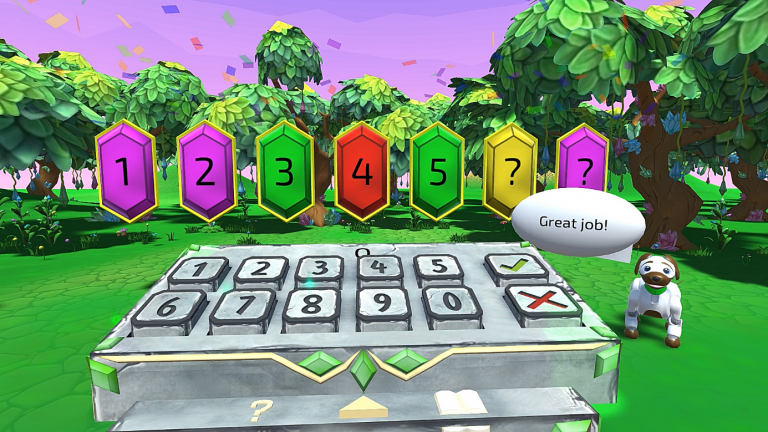
\includegraphics[width=0.5\textwidth]{03.EstudioProblema/01.EstadoArte/00.Figuras/07.kojis_quest.png}
    \caption{Juego de cálculo en Koji's Quest. \cite{EA_img_kojisQuest}}
    \label{fig:EA_kojisQuest}
\end{figure}

\subsubsection{Virtuleap}

Virtuleap ofrece su aplicación Enhance que es una compilación de juegos brain training en RV (figura \ref{fig:EA_enhance}). Estos juegos abarcan una amplia selección de habilidades cognitivas: memoria, resolución de problemas, orientación espacial, control motor y cognición auditiva entre otras. Su catálogo de juegos se incrementa mes a mes, lo que hace a Enhance una herramienta muy valiosa en el entrenamiento cognitivo con realidad virtual. \cite{EA_ent_virtuleap}


\begin{figure}
  \centering
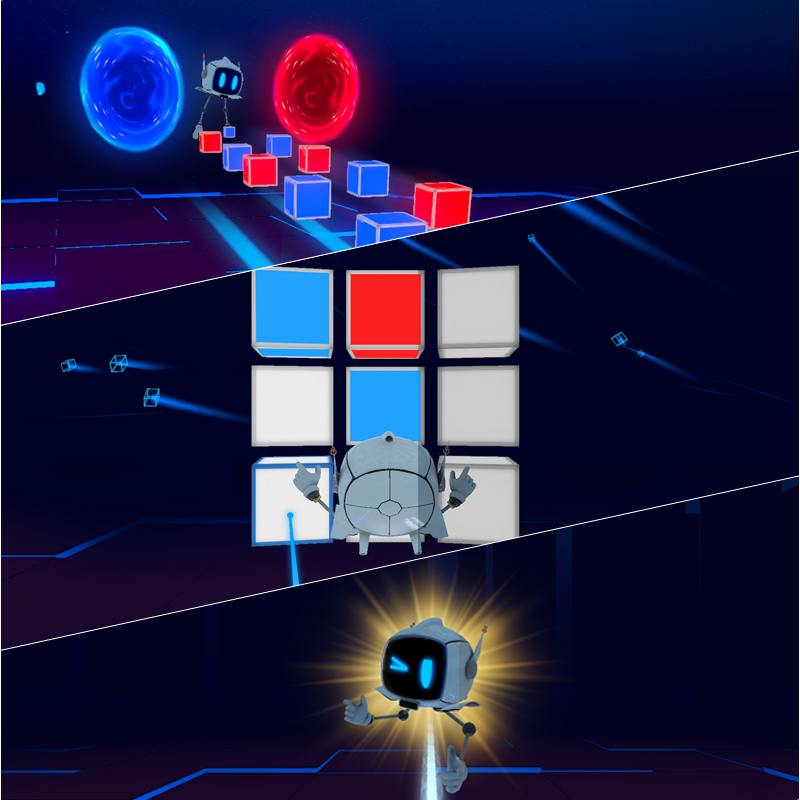
\includegraphics[width=0.5\textwidth]{03.EstudioProblema/01.EstadoArte/00.Figuras/08.enhance.jpg}
    \caption{Demostración de Enhance. \cite{EA_img_enhance}}
    \label{fig:EA_enhance}
\end{figure}

\section{Realidad Virtual}

La realidad virtual es una tecnología que busca simular objetos, entornos o cualquier sensación de modo que parezcan reales para un usuario. Para alcanzar este objetivo se necesita que el usuario tenga la mayor inmersión posible dentro del entorno virtual, para ello se suelen utilizar gafas o cascos de realidad virtual, conocidos en inglés por las siglas HMD (Head Mounted Display).

Estos dispositivos proveen al usuario de visión estereoscópica que permite ver las imágenes recibidas en 3D, así como audio tridimensional basado en el entorno virtual u otras sensaciones hápticas mediante motores de vibración incorporados en el dispositivo. 

A pesar de que los HMD son el elemento principal de la RV, tienen gran importancia también otros dispositivos que permiten la interacción del usuario con el entorno virtual, como son los mandos de juego que dan presencia en el entorno a las manos del usuario o guantes con retroalimentación que permiten a jugador sentir mediante el tacto, los objetos simulados dentro del entorno.

Actualmente la realidad virtual es una tecnología muy utilizada en una gran variedad de campos debido a la capacidad de reproducir entornos o situaciones similares a la realidad que se pueden utilizar tanto para estudio como diversión. Se utiliza por ejemplo, para simular casos médicos donde personal sanitario puede practicar cirugías sin riesgo para un paciente real, pudiendo incluso simular una representación real de un paciente concreto que previamente haya sido estudiado y escaneado para plasmar la realidad en el entorno virtual. 

Aunque la realidad virtual es una tecnología en alza en la actualidad, esta idea data de muchos años antes de la invención de los computadores, principalmente durante el siglo XIX en Europa, aunque el primer gran salto en la inmersión y el realismo de las obras artísticas surgió durante el Renacimiento.




\subsection{Renacimiento}

El arte de la Edad Media estaba caracterizado por su representación rudimentaria de formas tridimensionales, apareciendo completamente planas (véase la ilustración del poema 'Roman de la Rose' del siglo XIII presentada en la figura \ref{fig:EA_roman}, dificultando la inmersión del espectador por su gran diferencia con el mundo en el que vive.

Esto cambió durante el Renacimiento en Europa con la introducción de la perspectiva en la pintura. La perspectiva es una técnica geométrica para representar volúmenes en un espacio 3D mediante el uso de una línea de horizonte y uno o varios puntos de fuga.

La línea de horizonte representa objetos a una distancia infinita del espectador, y el resto de los objetos de la escena escalaran en tamaño dependiendo de su cercanía al punto de vista. Las líneas paralelas a la visión del espectador convergen en alguno de los puntos de fuga existentes, creando una deformación aparente en el objeto, pero que consigue una visión más realista del mismo. Esta técnica es especialmente visible en pinturas como 'La última cena' de Leonardo Da Vinci (figura \ref{fig:EA_cenaLeonardo}) o la 'Entrega de las llaves a San Pedro' de Pietro Perugino (figura \ref{fig:EA_llaves}).



\begin{figure}
  \centering
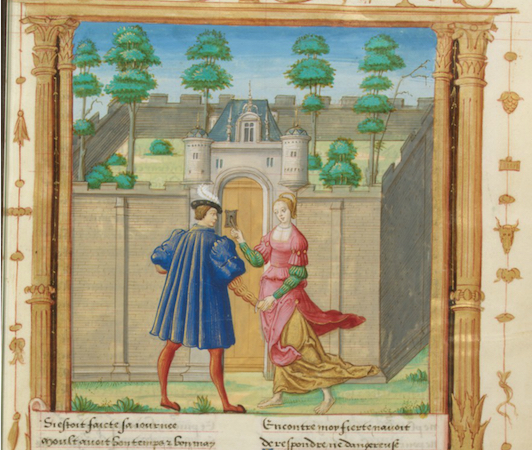
\includegraphics[width=0.5\textwidth]{03.EstudioProblema/01.EstadoArte/00.Figuras/09.renacimiento_roman_rose.jpg}
    \caption{Roman de la Rose. \cite{EA_img_roman}}
    \label{fig:EA_roman}
\end{figure}


\begin{figure}
\centering
\begin{minipage}{.5\textwidth}
  \centering
  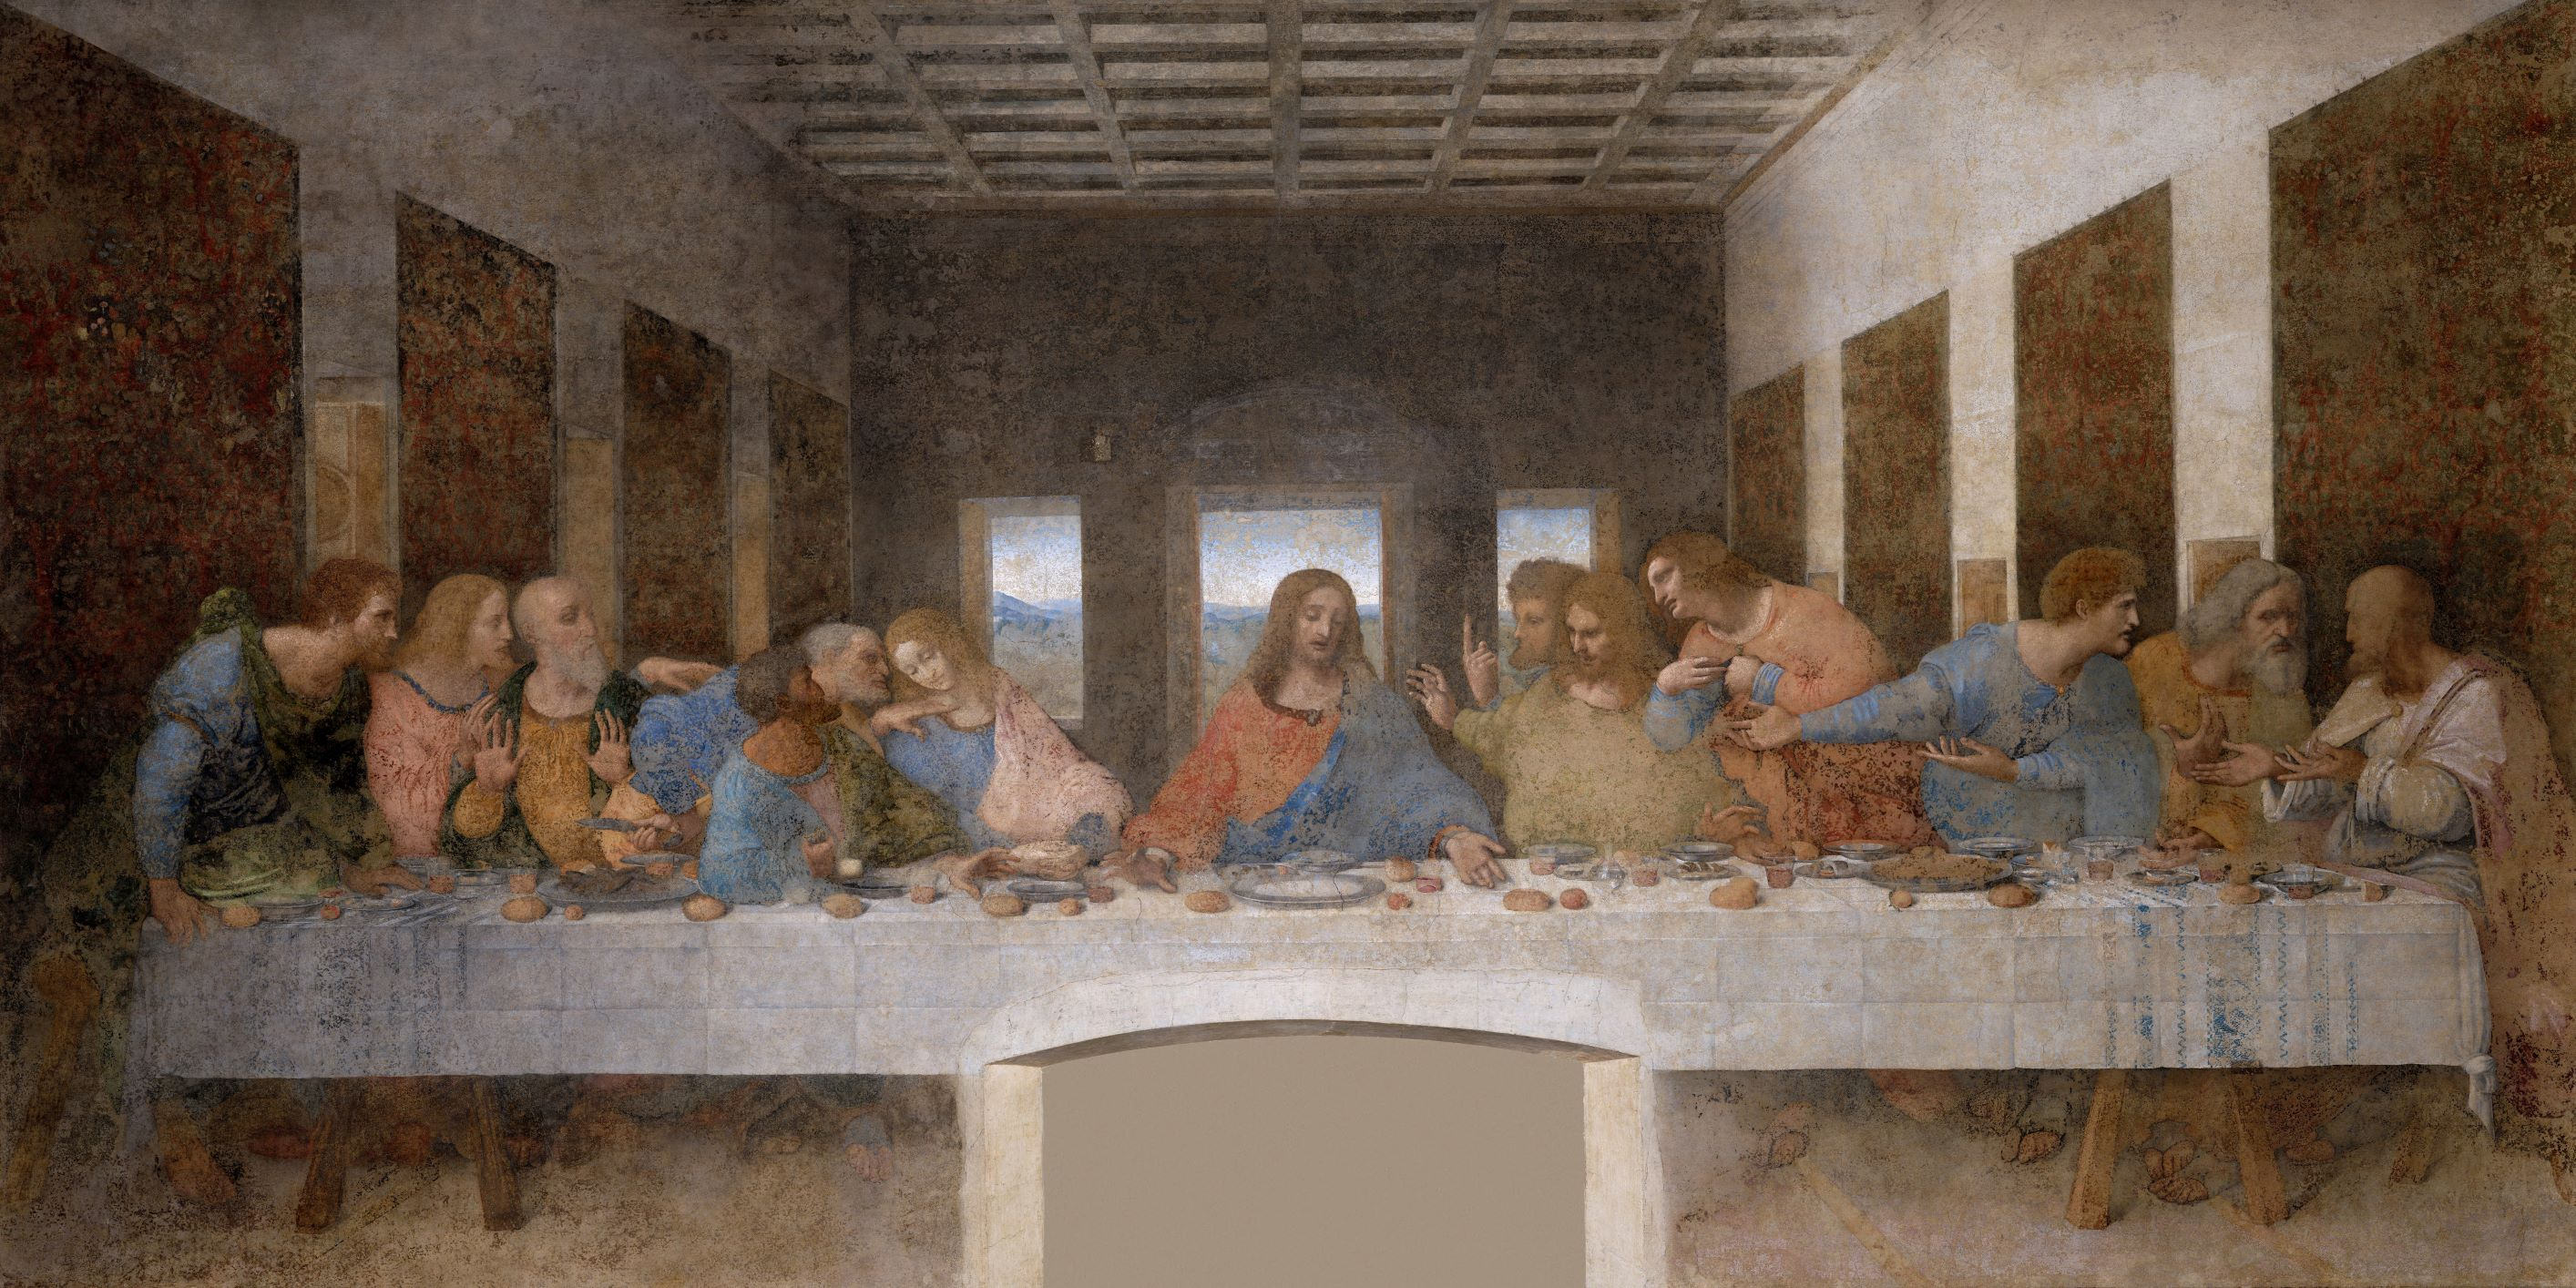
\includegraphics[width=.9\linewidth]{03.EstudioProblema/01.EstadoArte/00.Figuras/10.renacimiento_ultima_cena.jpg}
  \captionof{figure}{La última Cena. Leonardo Da Vinci. \cite{EA_img_cenaLeonardo}}
  \label{fig:EA_cenaLeonardo}
\end{minipage}%
\begin{minipage}{.5\textwidth}
  \centering
  \includegraphics[width=.9\linewidth]{03.EstudioProblema/01.EstadoArte/00.Figuras/11.renacimiento_llaves_san_pedro.jpg}
  \captionof{figure}{Entrega de las llaves a San Pedro. Pietro Perugino. \cite{EA_img_llaves}}
  \label{fig:EA_llaves}
\end{minipage}
\end{figure}






\subsection{Siglo XIX}

Durante el siglo XIX se populariza en Europa el uso de imágenes panorámicas que ocupan los 360º de visión horizontal del espectador para transportarlo al lugar o evento representado. Comenzaron a crearse edificios de ocio dedicados a la presentación de imágenes panorámicas en los que los espectadores eran situados en el centro de una sala circular desde donde podían contemplar una o varias pinturas, normalmente de paisajes naturales, ciudades y zonas urbanas, así como grandes batallas militares, siendo una de las más populares el panorama de Londres de Robert Barker presentado en la figura \ref{fig:EA_london}.

El pintor Robert Barker fue el gran impulsor de este tipo de entretenimiento con su Rotunda en Leicester Square (véase figura \ref{fig:EA_rotunda}), donde exponía sus pinturas.



\begin{figure}
  \centering
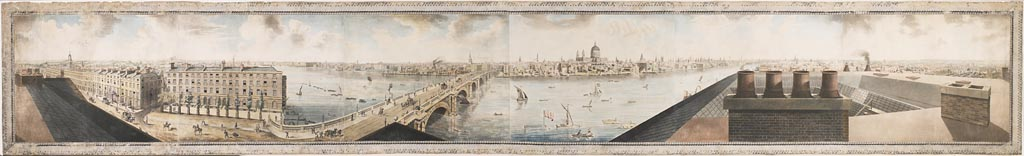
\includegraphics[width=0.9\textwidth]{03.EstudioProblema/01.EstadoArte/00.Figuras/12.panorama_london.jpg}
    \caption{Panorama de Londres. \cite{EA_img_london}}
    \label{fig:EA_london}
\end{figure}

\begin{figure}
  \centering
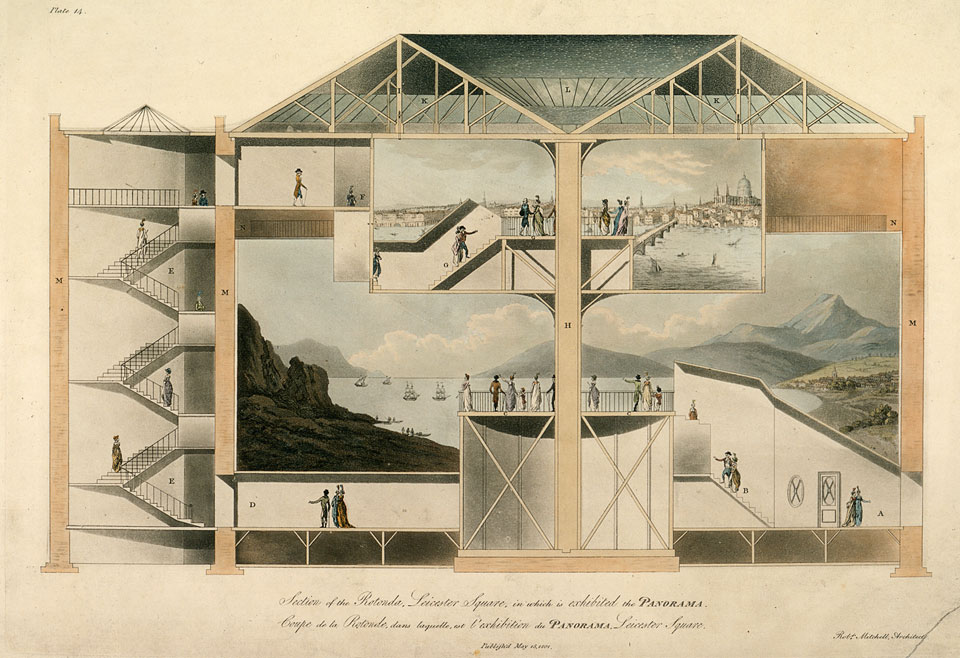
\includegraphics[width=0.5\textwidth]{03.EstudioProblema/01.EstadoArte/00.Figuras/13.panorama_rotunda.jpg}
    \caption{Sección de la Rotunda en Leicester Square. \cite{EA_img_rotunda}}
    \label{fig:EA_rotunda}
\end{figure}


\label{par:estadoArte:estereoscopio}
En 1836 se descubre que el cerebro humano procesa por separado las imágenes de ambos ojos para crear una única imagen con profundidad debido a las ligeras diferencias entre la visión de cada ojo. Esto lleva al nacimiento de los primeros visores de imágenes estereoscópicas (figura \ref{fig:EA_estereoscopio}). En estos visores era posible insertar una serie de diferentes tarjetas que contenían dos imágenes tomadas con una cámara estereoscópica y permitían disfrutar de su visualización con una inmersión mayor a lo común para la época.


\begin{figure}
  \centering
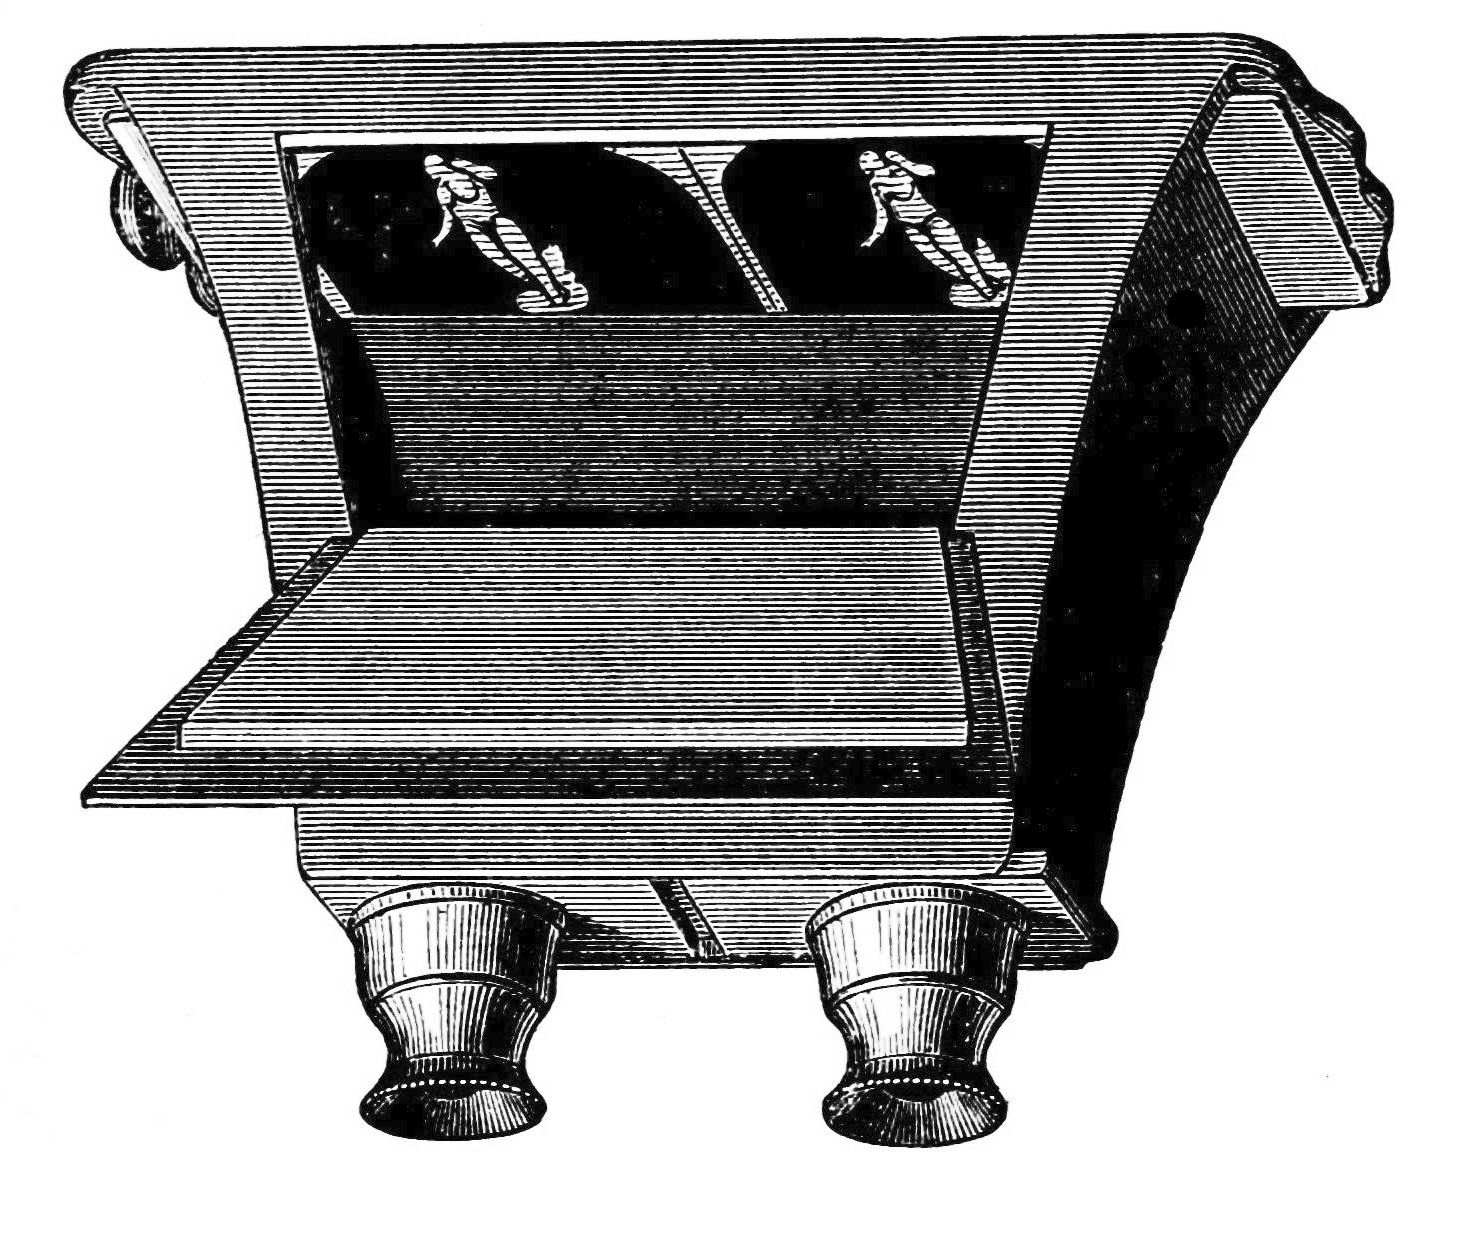
\includegraphics[width=0.5\textwidth]{03.EstudioProblema/01.EstadoArte/00.Figuras/14.panorama_estereoscopico.jpg}
    \caption{Estereoscopio de David Brewster. \cite{EA_img_estereoscopio}}
    \label{fig:EA_estereoscopio}
\end{figure}




\subsection{Headsight}

En 1960 Morton Heilig creó el primer visor que se colocaba en la cabeza y permitía ver una película estereoscópica. Este dispositivo era muy limitado, pero en el año siguiente (1961) Philco Corporation creó el primer casco de realidad virtual con sensores de movimiento, el Headsight (figura \ref{fig:EA_headsight}). Headsight fue desarrollado para un uso militar y permitía al usuario controlar la rotación de una cámara de vigilancia según los movimientos de su cabeza mediante el uso de sensores magnéticos que controlaban la posición del visor.



\begin{figure}[H]
  \centering
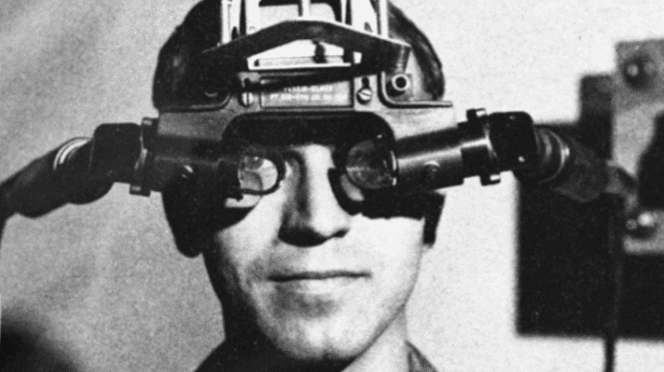
\includegraphics[width=0.5\textwidth]{03.EstudioProblema/01.EstadoArte/00.Figuras/15.headsight.png}
    \caption{Headsight de Philco Corporation. \cite{EA_img_headsight}}
    \label{fig:EA_headsight}
\end{figure}



\subsection{Espada de Damocles}

En 1968 se dio un paso más hacia la realidad virtual que se conoce hoy en día. Ivan Sutherland y Bob Sproull tomaron la idea del Headsight y la transformaron de forma que en lugar de estar conectado una cámara de vigilancia se conectaría a un ordenador que generaría gráficos tridimensionales sencillos. Este dispositivo era tan grande y pesado que necesitaba ser sostenido del techo sobre el usuario, dándole así su nombre en referencia a la leyenda de Damocles en la cultura griega clásica. En la figura \ref{fig:EA_damocles} se puede comprobar el tamaño del dispositivo y su colocación sobre el usuario.


\begin{figure}[H]
  \centering
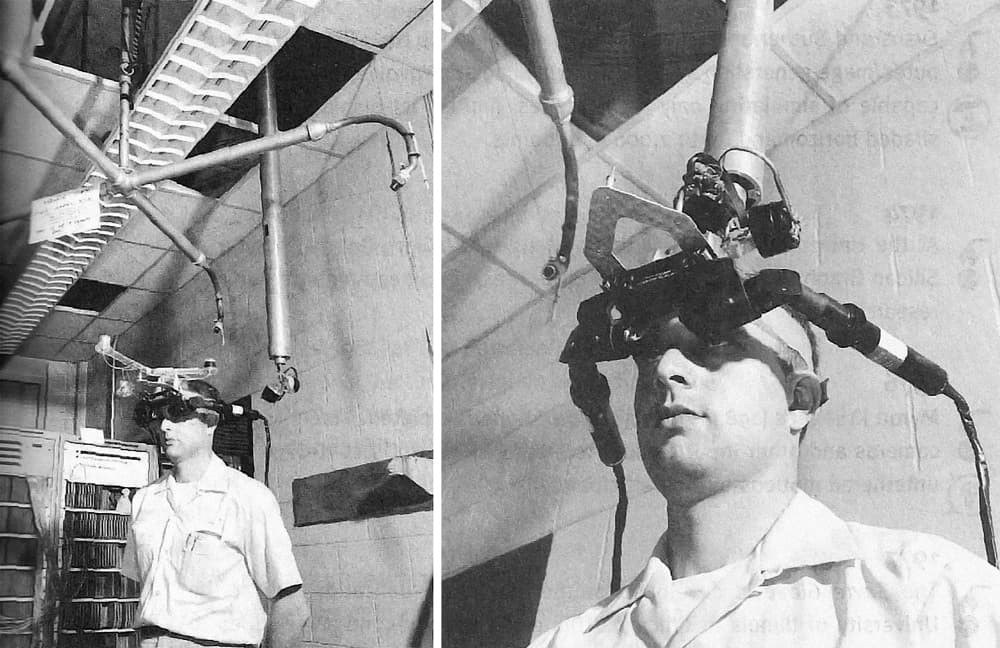
\includegraphics[width=0.5\textwidth]{03.EstudioProblema/01.EstadoArte/00.Figuras/16.damocles.jpg}
    \caption{Espada de Damocles de Ivan Sutherland y Bob Sproull. \cite{EA_img_damocles}}
    \label{fig:EA_damocles}
\end{figure}


\subsection{Realidad virtual}

A pesar de todos estos avances en la reproducción de una realidad artificial, no se disponía de un nombre y fue en 1987 cuando el término realidad virtual es definido por Jaron Lanier un informático y compositor estadounidense. Tras fundar una compañía llamada Visual Programming Lab, diseñó y desarrolló los que serían los primeros dispositivos de realidad virtual disponibles para ser adquiridos por el público: el EyePhone y el Dataglove, un visor y un guante para interactuar con el espacio virtual.

Pese al gran avance que suponen estos productos, la tecnología aún tenía mucho por mejorar. El sistema del EyePhone junto con el ordenador necesario para generar las imágenes del mundo virtual costaban hasta 250.000 dólares, y aun así solo eran capaces de alcanzar una tasa de imágenes de 5 fotogramas por segundo, una cifra insuficiente para ofrecer una experiencia fluida al usuario.

Este visor contenía elementos nunca vistos en el ámbito de la realidad virtual. Utilizaba sensores capaces de reconocer las expresiones faciales del usuario, todos los sonidos eran procesados por el ordenador para darles un efecto 3D de forma que su fuente se movía por el espacio dependiendo de los movimientos de la cabeza del usuario. El Dataglove solo era capaz de transmitir sensaciones hápticas al usuario si no que también actuaba como sensor, pudiendo generar en el espacio virtual un modelo de la mano del usuario que éste podía utilizar para interactuar con el ambiente.

A pesar de que este dispositivo fue el primero que se asemejaba a la visión actual de un visor de realidad virtual, requería de una gran potencia informática para la época, resultando en un producto demasiado caro y voluminoso, como se puede ver en la figura \ref{fig:EA_eyePhone}.




%\begin{figure}
%\centering
%\begin{minipage}{.5\textwidth}
%  \centering
%  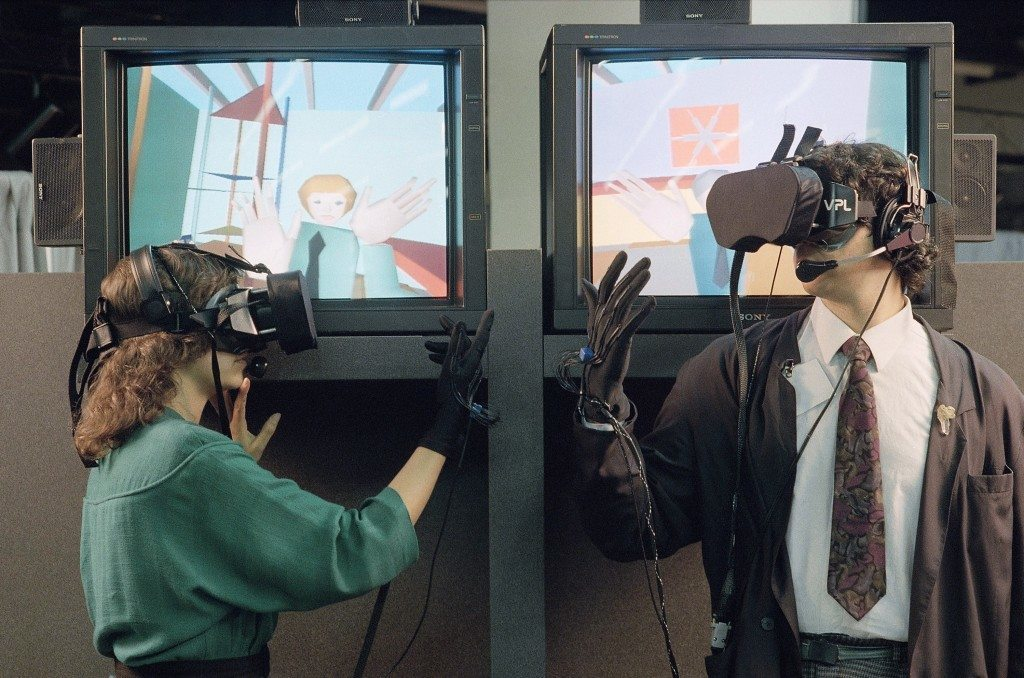
\includegraphics[width=.9\linewidth]{03.EstudioProblema/01.EstadoArte/00.Figuras/eyephone.jpg}
%  \captionof{figure}{Demostración de EyePhone y Dataglove.
%. \cite{EA_img_eyePhone}}
%  \label{fig:EA_eyePhone}
%\end{minipage}%
%\begin{minipage}{.5\textwidth}
%  \centering
%  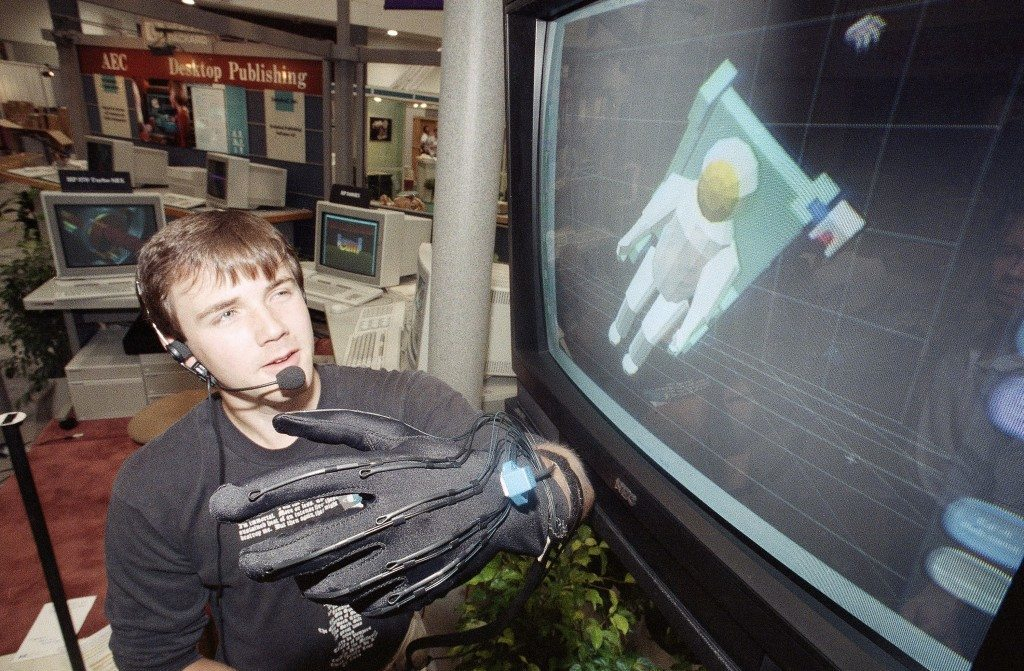
\includegraphics[width=.9\linewidth]{03.EstudioProblema/01.EstadoArte/00.Figuras/eyephoneDataglove.jpg}
%  \captionof{figure}{Dataglove siendo usado por Chad Leeper durante una conferencia.
%. \cite{EA_img_dataglobe}}
%  \label{fig:EA_dataglobe}
%\end{minipage}
%\end{figure}

\begin{figure}[H]
  \centering
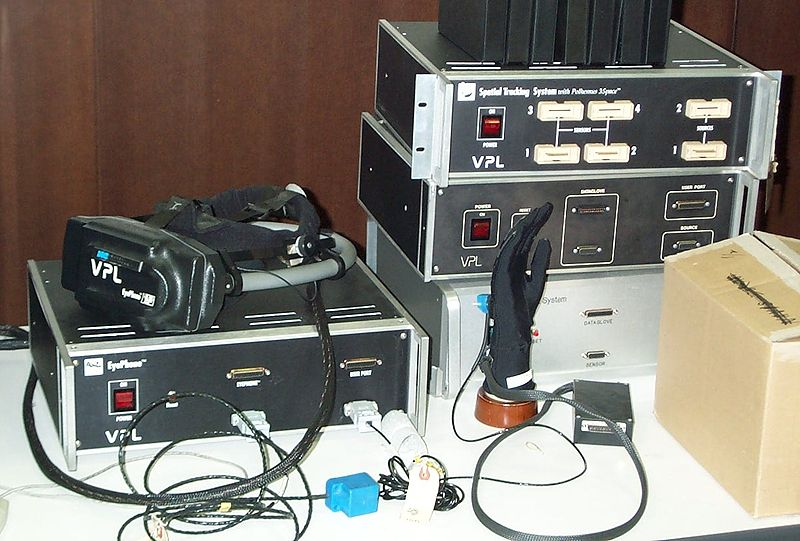
\includegraphics[width=0.5\textwidth]{03.EstudioProblema/01.EstadoArte/00.Figuras/17.eyephone_dataglove.jpg}
    \caption{Eyephone y Dataglove junto al sistema de seguimiento Polhemus en exposición Nissho Iwai en Tokio en 1999. \cite{EA_img_eyePhone}}
    \label{fig:EA_eyePhone}
\end{figure}


\subsection{Virtual Boy}

En 1995 la compañía de videojuegos japonesa Nintendo lanza al mercado su Virtual Boy, la primera consola portátil con gráficos verdaderamente tridimensionales (figura \ref{fig:EA_virtualBoy}). Esta consola prometía ser un gran éxito, pero acabó siendo un fracaso. Su precio, aun siendo más asequible que el EyePhone, seguía siendo elevado para lo que ofrecía: 180 dólares.

La Virtual Boy disponía de dos matrices lineales de láser de 1x224 que escaneaban constantemente el campo visual de cada ojo con la ayuda de dos espejos que oscilaban rápidamente. Por esto, la consola emitía un constante murmuro mientras estaba en uso.

La consola solo podía reproducir un único color, junto con el negro. Se escogió el color rojo por las características de los LED de este color: son más baratos y consumen menos energía que otros colores.

Esta consola utilizaba un procesador NEC V810 de arquitectura RISC y 32 bit a 20MHz, que era acompañado de 1MB de memoria RAM. La resolución efectiva de las pantallas era de 384x224 píxeles. Toda la consola era alimentada a partir de 6 pilas AA situadas en el mando.

Por desgracia, el uso prolongado de este dispositivo causaba dolores de cabeza y mareos, que, junto con su pequeña y básica selección de juegos (entre ellos, el más popular: Mario's Tennis, representado en la figura \ref{fig:EA_virtualBoyJuego}), llevaron a que la consola fuera descontinuada menos de un año después de su lanzamiento.



\begin{figure}
\centering
\begin{minipage}{.5\textwidth}
  \centering
  \includegraphics[width=.7\linewidth]{03.EstudioProblema/01.EstadoArte/00.Figuras/18.virtualboy.png}
  \captionof{figure}{Virtual Boy de Nintendo. \cite{EA_img_virtualBoy}}
  \label{fig:EA_virtualBoy}
\end{minipage}%
\begin{minipage}{.5\textwidth}
  \centering
  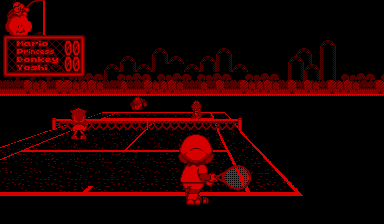
\includegraphics[width=.9\linewidth]{03.EstudioProblema/01.EstadoArte/00.Figuras/19.marios_tennis.png}
  \captionof{figure}{Mario's Tennis. Videojuego de Nintendo para Virtual Boy. \cite{EA_img_virtualBoyJuego}}
  \label{fig:EA_virtualBoyJuego}
\end{minipage}
\end{figure}



\subsection{Siglo XXI}

En los últimos años ha habido un crecimiento acelerado de la tecnología: los ordenadores han multiplicado su potencia y capacidad de procesamiento paralelo, los dispositivos móviles se han vuelto mucho más sofisticados que cualquier ordenador del siglo XX, las pantallas son capaces de reproducir millones de colores a altas frecuencias de refresco y el acceso a Internet de alta velocidad es algo común. Estos avances han hecho resurgir con más fuerza que nunca la realidad virtual, especialmente en el ámbito de los videojuegos.

En 2010, el joven empresario Palmer Luckey creó el prototipo de un casco de realidad virtual al que llamó Oculus Rift, véase la figura \ref{fig:EA_kitOculus}. Este dispositivo podía representar imágenes de alta resolución con un campo de visión de 90º, algo muy superior a lo existente hasta el momento. Dos años después, Oculus Rift logró financiación a partir de una campaña de micro financiación.


\begin{figure}
  \centering
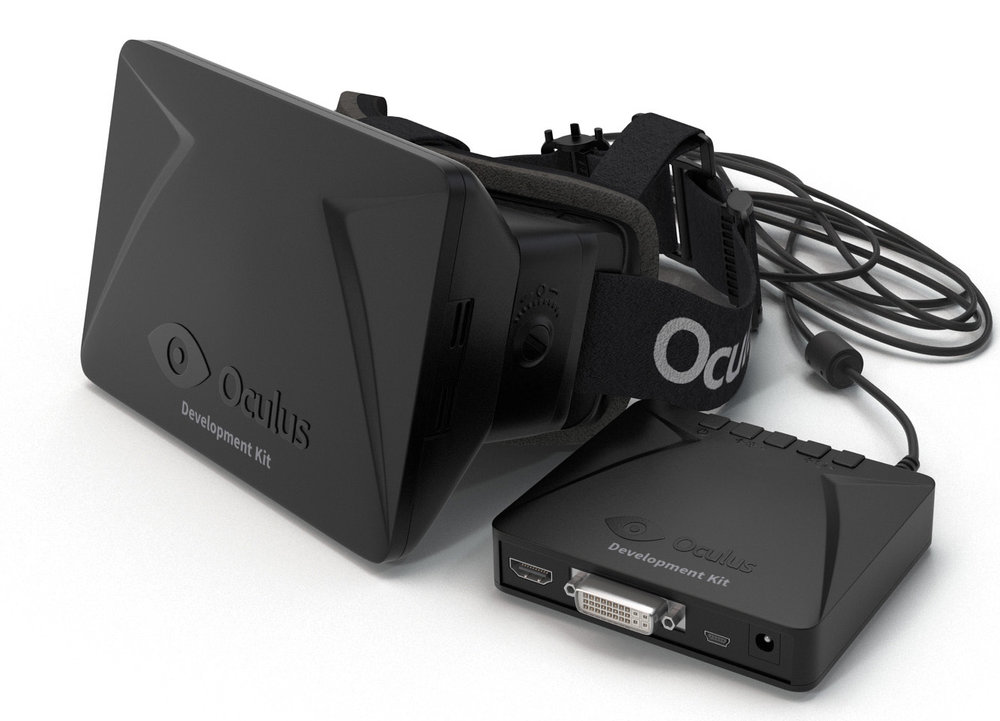
\includegraphics[width=0.5\textwidth]{03.EstudioProblema/01.EstadoArte/00.Figuras/20.oculus_rift_dk1.jpg}
    \caption{Primer kit de desarrollo de Oculus Rift. \cite{EA_img_kitOculus}}
    \label{fig:EA_kitOculus}
\end{figure}



Entre los años 2014 y 2015 se produjo un boom en la realidad virtual de consumo, apareciendo muchas alternativas para el público general:

\begin{itemize}
	\item{Sony anuncia PlayStation VR un casco de RV para su consola PlayStation 4. Figura \ref{fig:EA_psvr}.}

	\item{Samsung lanza al mercado su Samsung Gear VR, un visor que utiliza un smartphone (Samsung Galaxy) como centro de procesamiento y pantalla.}

	\item{Google produce las Google Cardboard, una alternativa barata que permite al usuario crear su propio visor y utilizar su propio dispositivo móvil con Android como pantalla. Figura \ref{fig:EA_cardboard}.}

\end{itemize}


\begin{figure}
  \centering
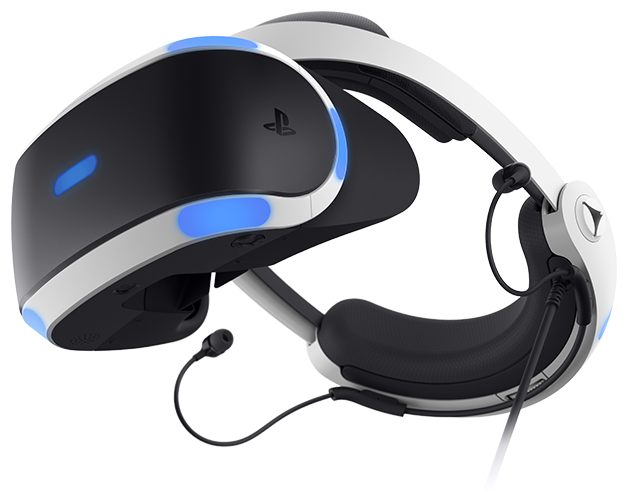
\includegraphics[width=0.5\textwidth]{03.EstudioProblema/01.EstadoArte/00.Figuras/21.psvr.png}
    \caption{PlayStation VR. \cite{EA_img_psvr}}
    \label{fig:EA_psvr}
\end{figure}

\begin{figure}
  \centering
\includegraphics[width=0.5\textwidth]{03.EstudioProblema/01.EstadoArte/00.Figuras/22.cardboard.jpg}
    \caption{Google Cardboard ensamblada. \cite{EA_img_cardboard}}
    \label{fig:EA_cardboard}
\end{figure}


Con la aparición de dispositivos capaces de reproducir contenido de realidad virtual, también fueron apareciendo videojuegos y otras experiencias para los mismos. La RV era ya una parte fundamental del ocio y los videojuegos.

En 2016 se lanza al mercado HTC Vive, un completo sistema de realidad virtual (véase figura \ref{fig:EA_vive}) producido en colaboración entre HTC y Valve, productores de hardware y software respectivamente. El HTC Vive pasó a ser el casco de RV de referencia en el sector: contaba con pantallas OLED de alta resolución (1080x1200 píxeles) y tasa de refresco de 90Hz que ofrecían un campo de visión de 110º, contaba con dos mandos de control táctiles con respuesta háptica, así como un sistema de sensores colocados en la habitación que permitían definir un espacio de juego de hasta 25 m2 en el que el jugador podía moverse libremente.


\begin{figure}
  \centering
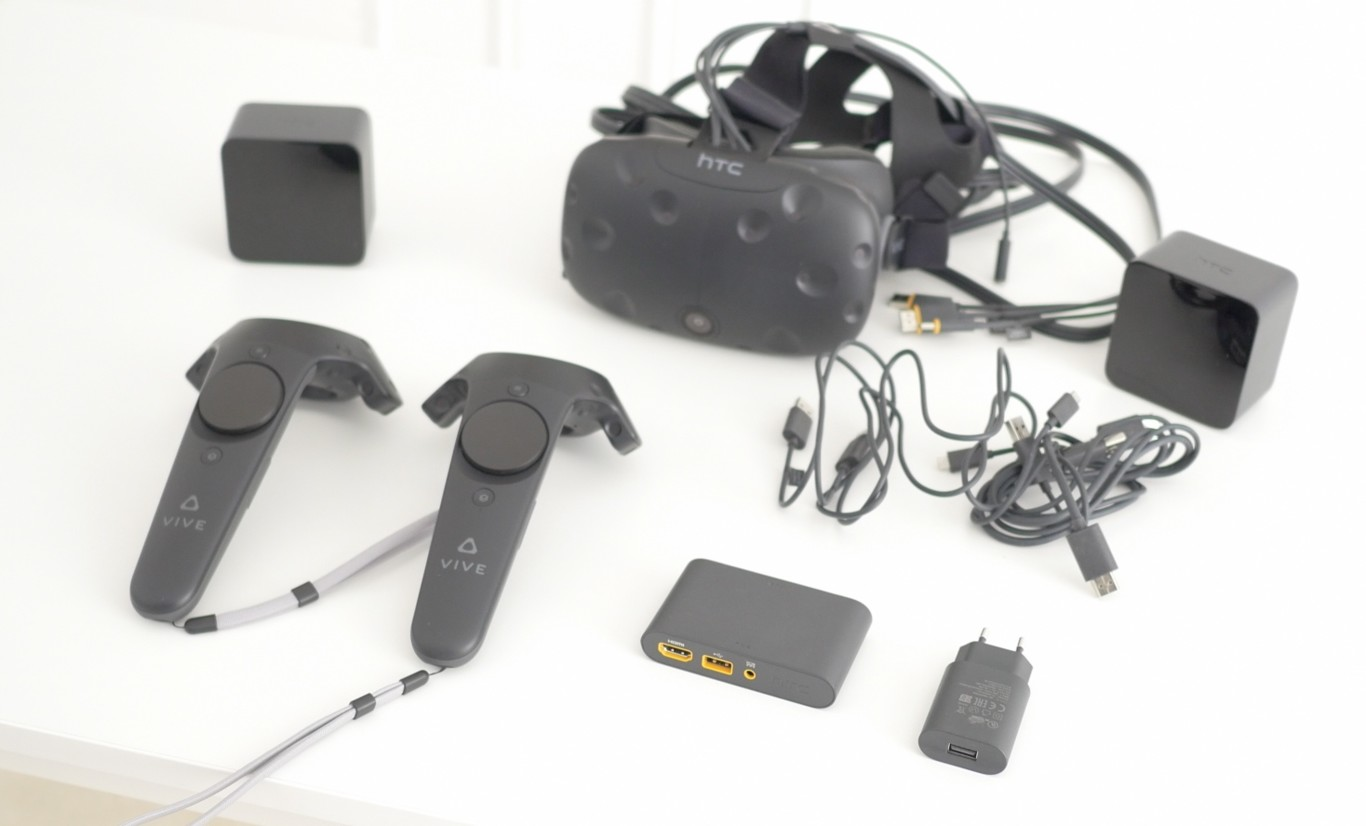
\includegraphics[width=0.5\textwidth]{03.EstudioProblema/01.EstadoArte/00.Figuras/23.htc_vive.jpeg}
    \caption{HTC Vive y todos sus complementos. \cite{EA_img_vive}}
    \label{fig:EA_vive}
\end{figure}


\subsection{Actualidad}


Actualmente, en el año 2019, la realidad virtual continua sin ser perfecta pero también continúa mejorando cada día. A pesar de no ser el más avanzado tecnológicamente, el dispositivo de Sony (PSVR) ha tenido una gran aceptación entre el público debido a su menor precio y especialmente a la enorme acogida de la consola PlayStation 4. Incluso 3 años después de su salida al mercado, y de las nuevas opciones disponibles, PSVR continúa siendo el dispositivo de realidad virtual más vendido en el mundo con 2.2 millones de unidades vendidas frente a los 1.7 millones de su competidor más cercano: Oculus.

En este último año, además, se han originado dos enfoques para la RV claramente diferenciados y liderados por dos empresas principalmente: Valve y Oculus.

En verano de 2019 Valve lanza al mercado un nuevo producto. Tras romper su alianza comercial con HTC, Valve desarrolla su propio visor de RV llamado Valve Index, mostrado en la figura \ref{fig:EA_index}. Este dispositivo mejora en todos los aspectos a su predecesor, el HTC Vive:


\begin{itemize}
	\item{Dispone de pantallas OLED de 1440x1600 píxeles con refresco de hasta 144Hz.}

	\item{Dos cámaras estereoscópicas situadas al frente del dispositivo permiten su uso durante el juego como cámaras de video o como sensores.}

	\item{Los mandos de control han sido mejorados y ahora son capaces de detectar movimientos de cada dedo individualmente gracias a sensores de proximidad.}
	
	\item{Las nuevas estaciones (sensores colocados en la habitación) ahora permiten un campo de juego de hasta 100m2 comparados con los 25m2 del HTC Vive.}

\end{itemize}


\begin{figure}
  \centering
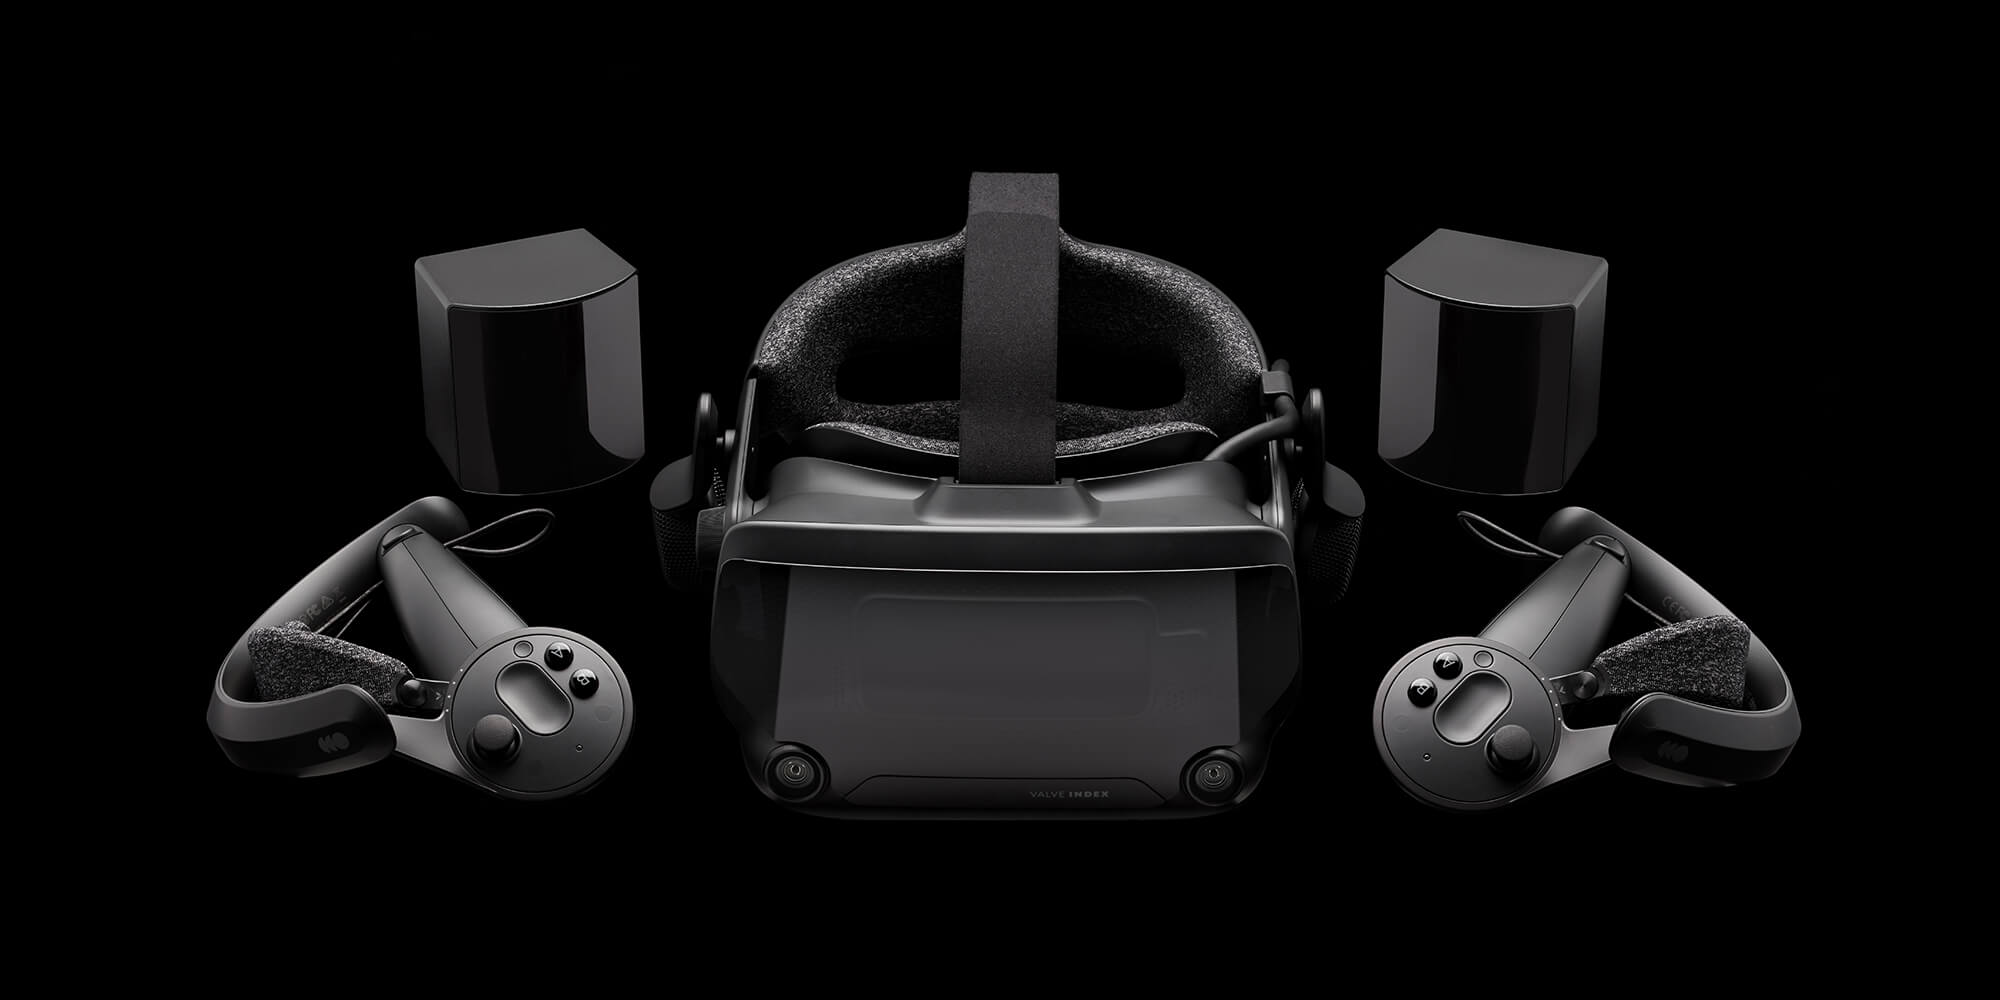
\includegraphics[width=0.5\textwidth]{03.EstudioProblema/01.EstadoArte/00.Figuras/24.valve_index.jpg}
    \caption{Kit de visor Valve Index junto a controles y estaciones base. \cite{EA_img_index}}
    \label{fig:EA_index}
\end{figure}



Pero todas estas mejoras conllevan un gran coste y el precio del kit completo asciende hasta 1080 euros en su lanzamiento. A este precio habrá que sumar el precio de un ordenador con capacidad suficiente para ejecutar los videojuegos tan demandantes que están diseñados para este dispositivo.

Por otra parte, Oculus lanza su nuevo producto un mes antes que el Valve Index, pero con una mentalidad completamente diferente: en lugar de buscar la máxima potencia e innovación tecnológica, se busca una mayor portabilidad y eficiencia manteniendo el coste bajo para que sea accesible por un mercado más amplio. Este nuevo dispositivo es el Oculus Quest. Este visor no se conecta a un ordenador para reproducir los videojuegos, si no que se trata de un visor de RV completamente independiente. Véase figura \ref{fig:EA_oculusQuest}.

Oculus Quest contiene un sistema Android personalizado que se ejecuta sobre un procesador ARM de 8 núcleos Cortex-A73 (4 núcleos Kryo 208 Gold a 2.45GHz y 4 Kryo 280 Silver a 1.9GHz) y un procesador gráfico Adreno 540, que están acompañados de 4GB de memoria RAM y hasta 128GB de almacenamiento. Tiene dos pantallas OLED de 1440x1600 píxeles similares a las del Valve Index, pero funcionan solo 72Hz.


\begin{figure}
  \centering
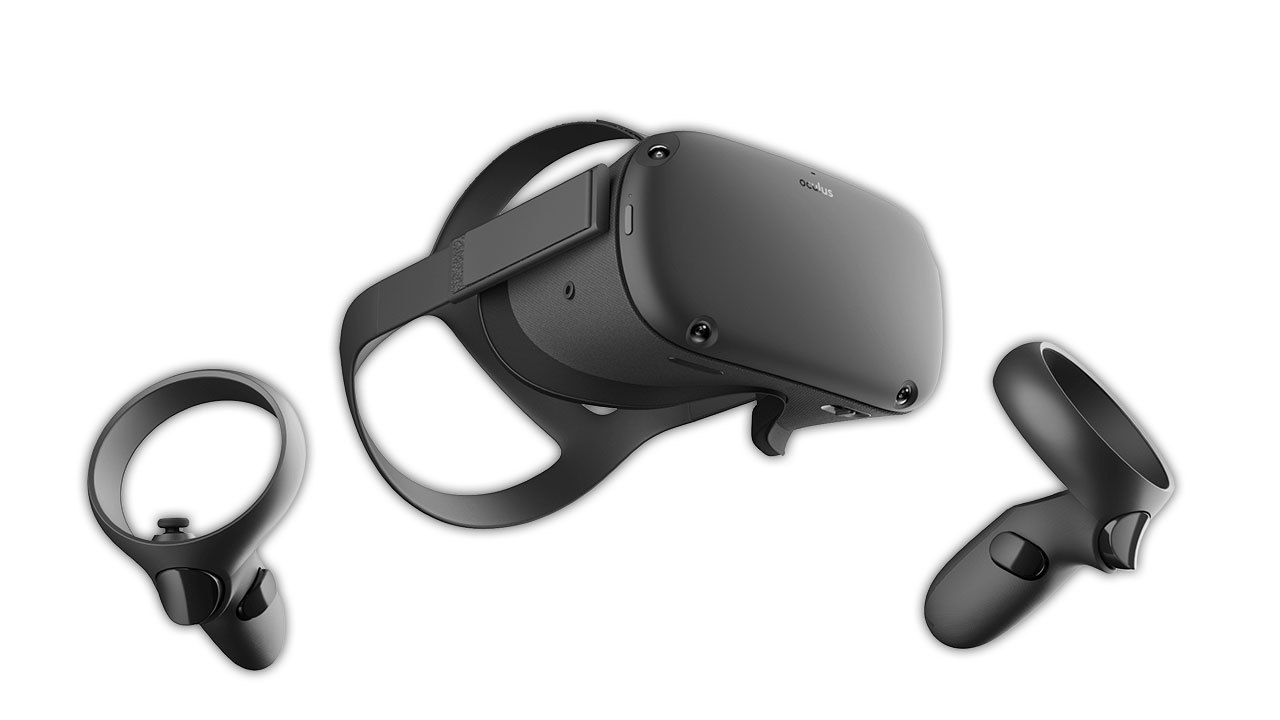
\includegraphics[width=0.5\textwidth]{03.EstudioProblema/01.EstadoArte/00.Figuras/25.meta_quest_2.jpg}
    \caption{Oculus Quest. \cite{EA_img_oculusQuest}}
    \label{fig:EA_oculusQuest}
\end{figure}


Este dispositivo no depende de estaciones de sensores fijas en la habitación ya que es capaz de generar la zona de juego a partir de los sensores que lleva incorporados el propio visor. Debido a esto aparecen nuevas restricciones en los mandos: para que estos funcionen de forma adecuada deberán estar situados delante del visor, si el usuario hace un movimiento demasiado amplio, los mandos saldrán de la zona captada por los sensores y dejarán de ser reconocidos.

Pese a ser un visor más limitado que el Valve Index, la portabilidad y precio del Oculus Quest hacen que sea uno de los visores de RV más para tener en cuenta en la actualidad.





\section{Motores de videojuegos}

Para diseñar y desarrollar videojuegos, ya sean de tipo brain training o cualquier otro, se utiliza habitualmente un motor de juego.

Un motor de juego es un entorno de trabajo o framework que contiene funcionalidades básicas para la creación de videojuegos como: un motor de físicas, renderizado de gráficos, gestor de comunicación en red o comunicaciones a bajo nivel con el hardware en el que se ejecutará el videojuego. Por tanto, un motor de juego provee de una base sobre la que desarrollar un videojuego de forma más ágil, ahorrando tiempo, esfuerzo y dinero.

\subsection{Unity}

Es un motor capaz de crear videojuegos multiplataforma de multitud de géneros de manera sencilla. Es el motor más utilizado por desarrolladores independientes debido a su bajo coste y a su gran comunidad de desarrolladores online y su gran documentación. Figura \ref{fig:EA_interfazUnity}.


\begin{figure}[H]
  \centering
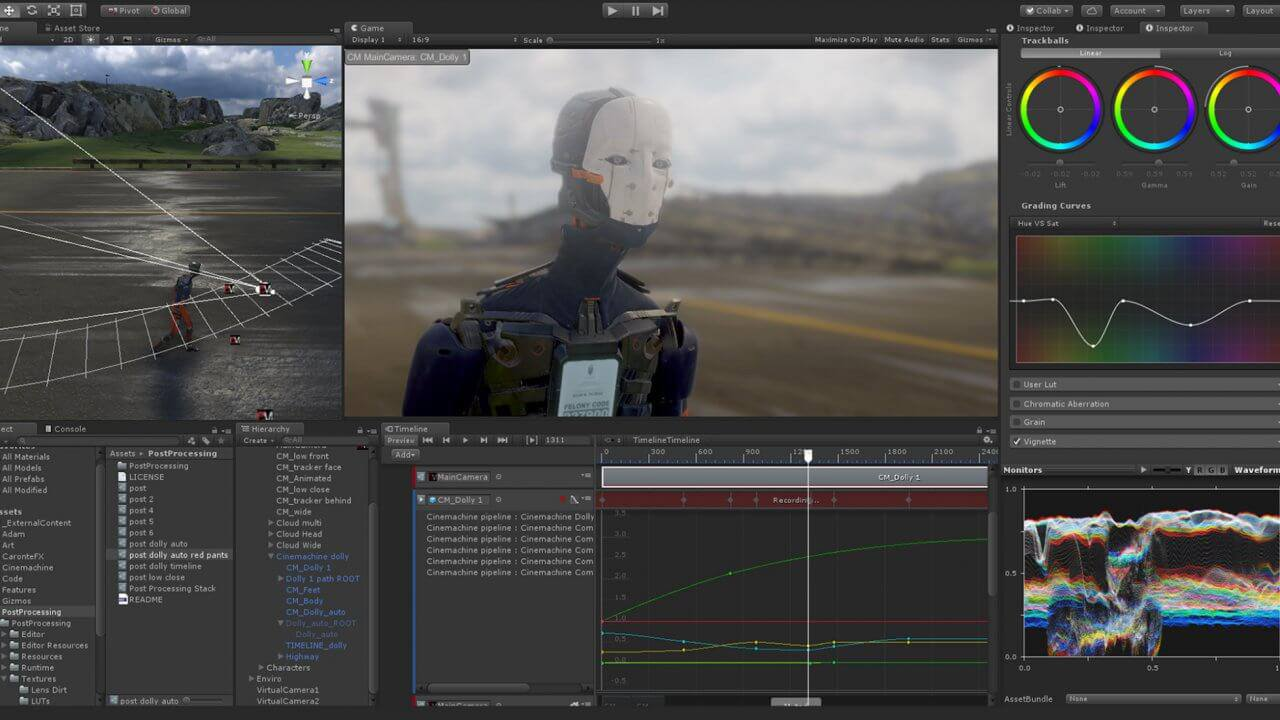
\includegraphics[width=0.8\textwidth]{03.EstudioProblema/01.EstadoArte/00.Figuras/26.interfaz_unity.jpg}
    \caption{Interfaz de Unity. \cite{EA_img_interfazUnity}}
    \label{fig:EA_interfazUnity}
\end{figure}


Destaca en la creación de videojuegos para plataformas móviles. Con este motor se ha desarrollado juegos como Ori and the Blind Forest, Hollow Knight, Monument Valley 2 (figura \ref{fig:EA_monumentValley}), Kerbal Space Program o Firewatch.

Unity cuenta con un plan personal completamente gratuito y libre de regalías. Pero en caso de que la recaudación del juego supere los 100.000 dólares al año se deberá adquirir un plan de pago mensual de entre 40 y 150 dólares. En caso de superar los 200.000\$ de ingresos o contar con más de 3 trabajadores, se deberá contratar un plan empresarial propuesto por Unity.





\begin{figure}[H]
  \centering
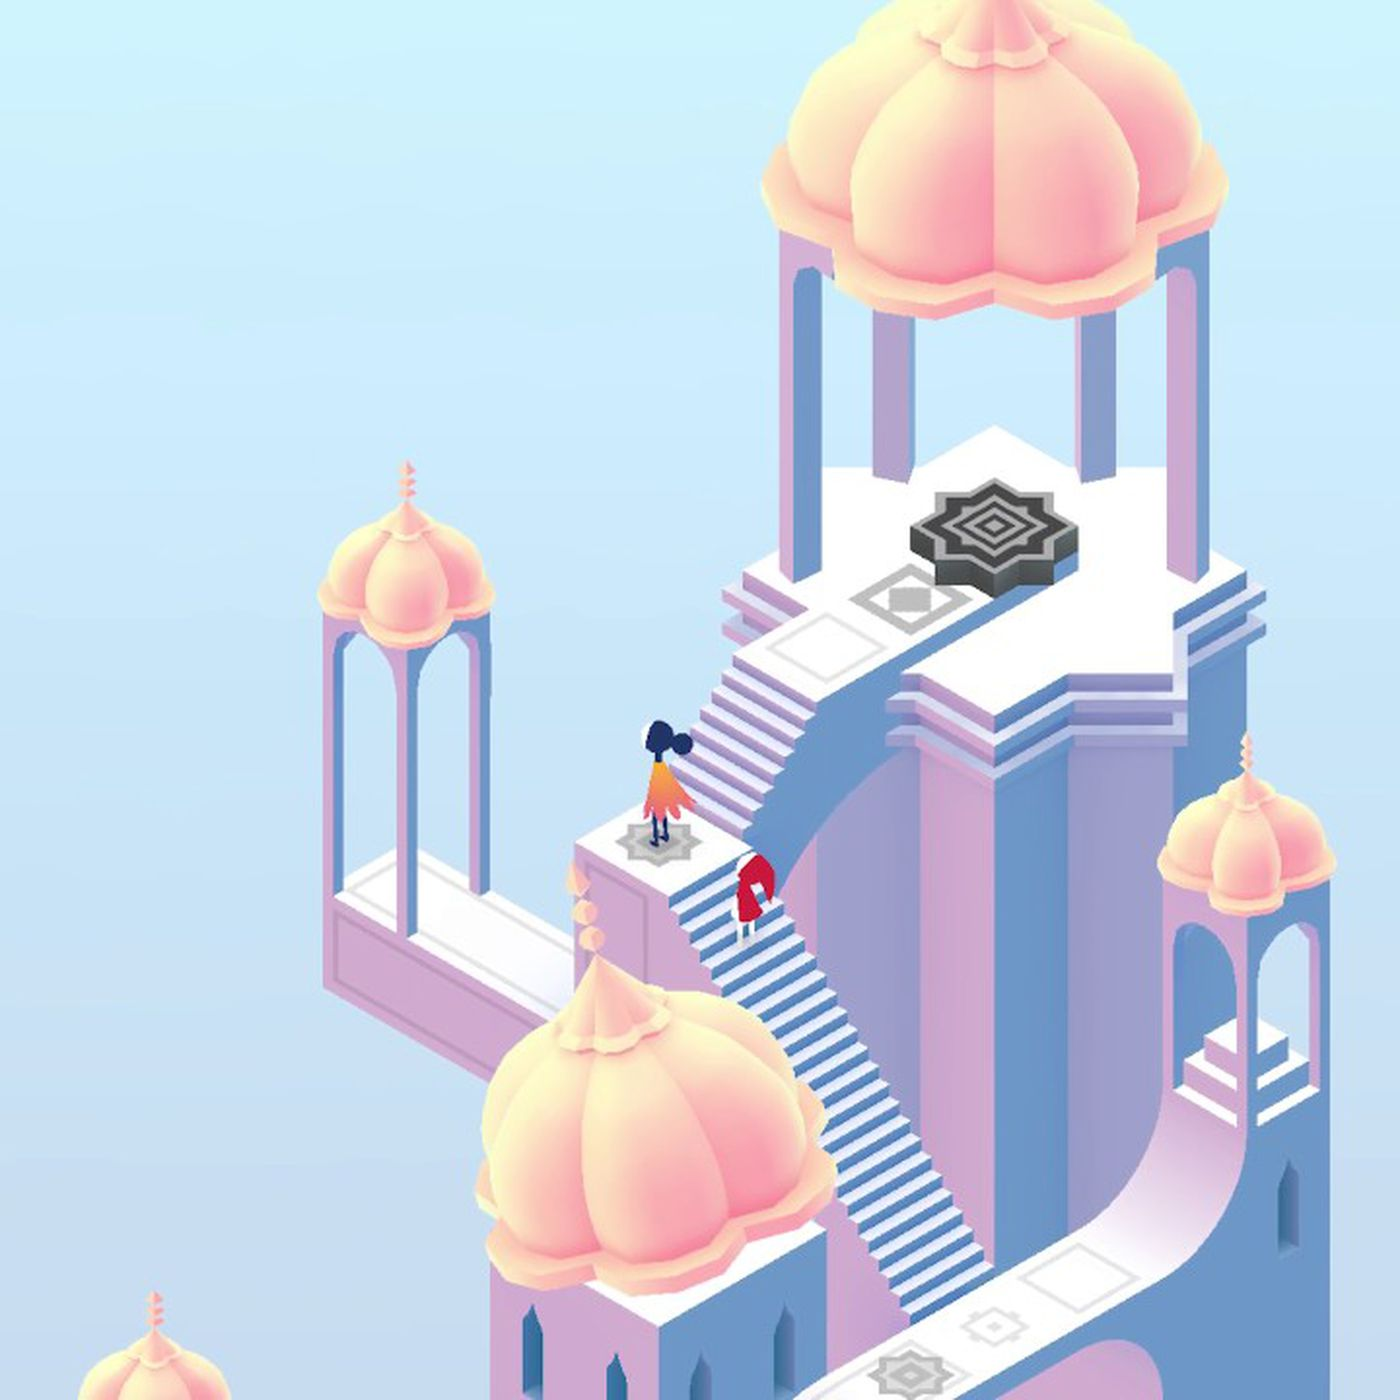
\includegraphics[width=0.6\textwidth]{03.EstudioProblema/01.EstadoArte/00.Figuras/27.monument_valley_2.jpg}
    \caption{Monument Valley 2. \cite{EA_img_monumentValley}}
    \label{fig:EA_monumentValley}
\end{figure}


\subsection{Unreal Engine}

Actualmente es uno de los motores más utilizados por su potencia y acabados gráficos, así como permitir trabajar para distintas plataformas, entre ellas PC, PS4, Xbox One, Nintendo Switch, Android o iOS. Fue creado por la empresa Epic Games, desarrolladora de juegos como Fortnite y la serie Unreal. Figura \ref{fig:EA_interfazUnreal}.

\begin{figure}[H]
  \centering
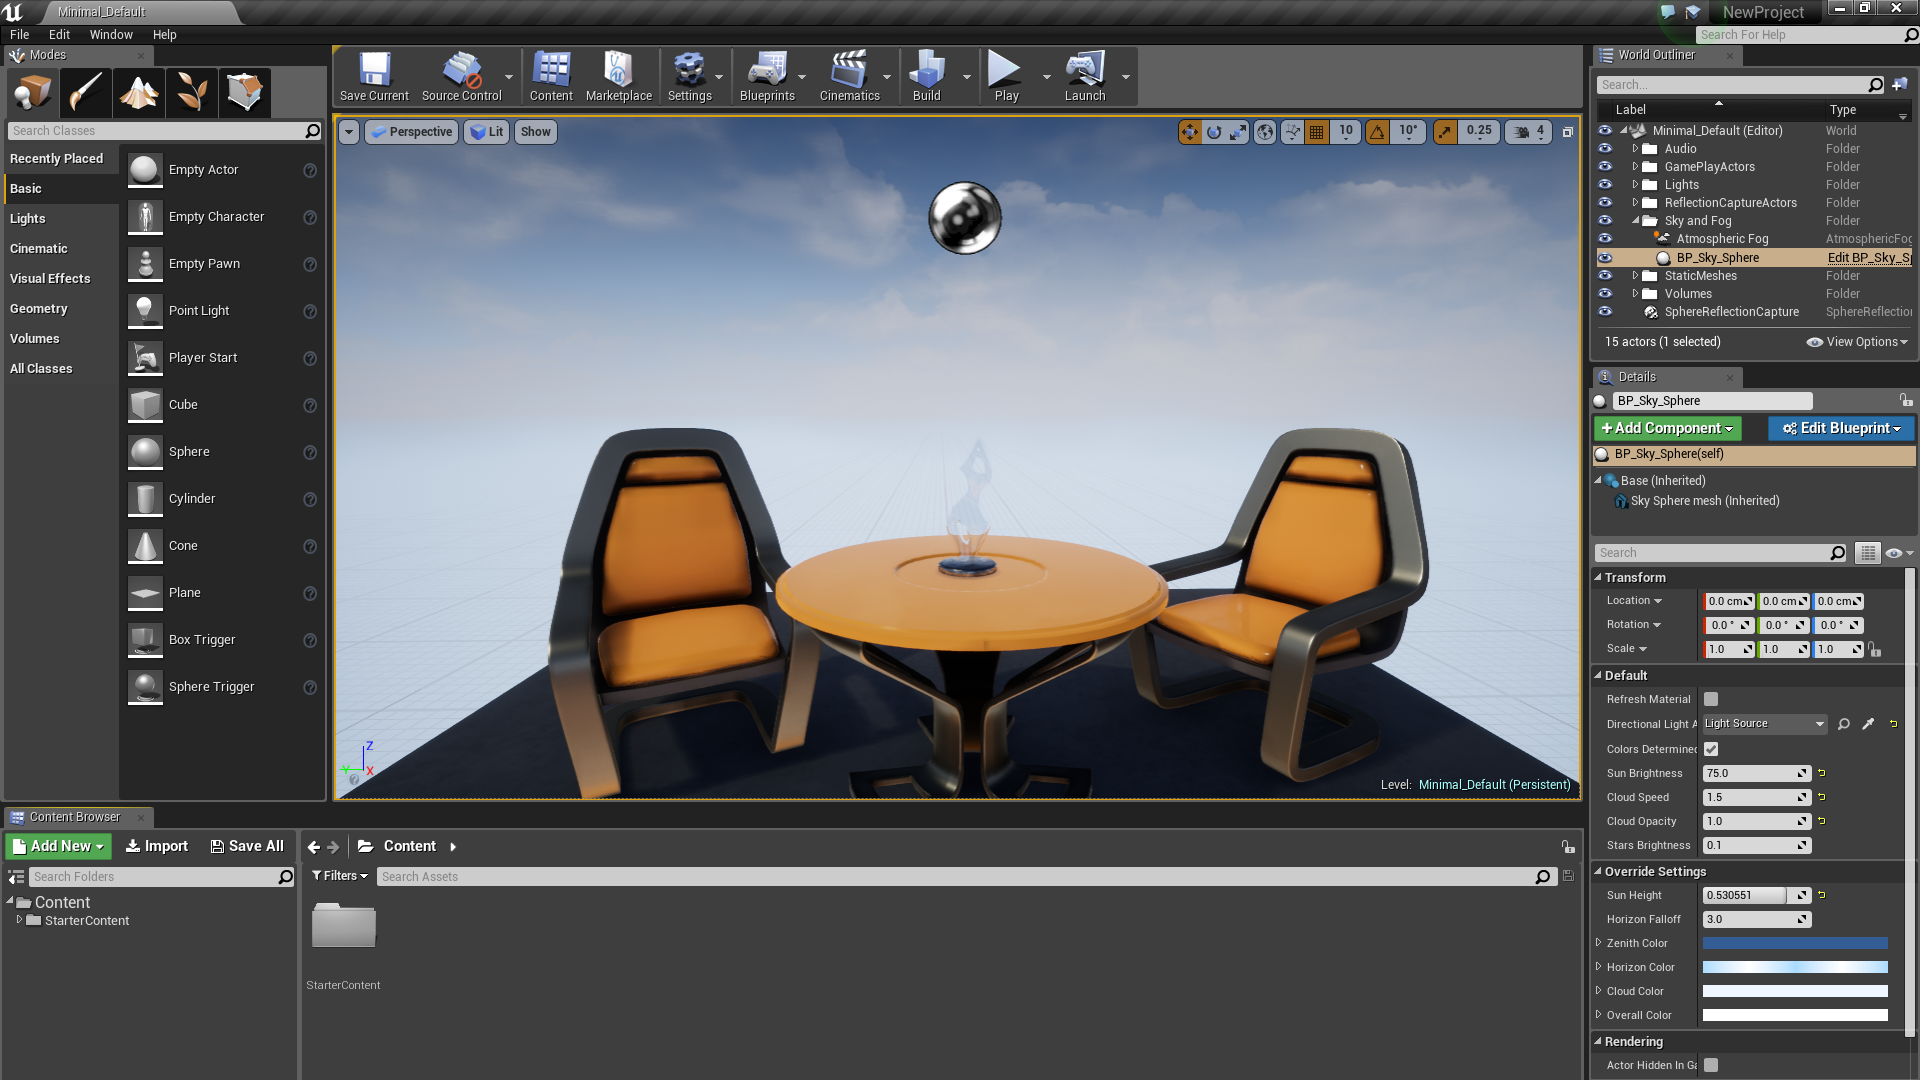
\includegraphics[width=0.8\textwidth]{03.EstudioProblema/01.EstadoArte/00.Figuras/28.interfaz_unreal.png}
    \caption{Interfaz de Unreal Engine 4. \cite{EA_img_interfazUnreal}}
    \label{fig:EA_interfazUnreal}
\end{figure}

Unreal Engine permite un elevado grado de personalización, lo que hace que pueda usarse para crear juegos de multitud de géneros diferentes: Aventura, FPS, lucha 2D, puzles, etc.

Este motor ha sido utilizado para crear los videojuegos de la saga Gears of War, Bioshock, Kingdom Hearts III y Fortnite (figura \ref{fig:EA_fortnite}) entre muchos otros.

Este motor presenta un modelo de negocio basado en regalías, de modo que su uso es completamente gratuito, pero a cambio Epic Games recibirá un 5\% de los ingresos del juego en caso de que este supere los 3000 dólares de beneficio en un trimestre.




\begin{figure}[H]
  \centering
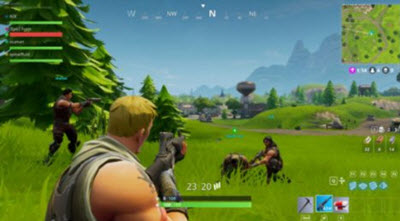
\includegraphics[width=0.8\textwidth]{03.EstudioProblema/01.EstadoArte/00.Figuras/29.fortnite.jpg}
    \caption{Visión del jugador durante una partida de Fortnite. \cite{EA_img_fortnite}}
    \label{fig:EA_fortnite}
\end{figure}





\subsection{Game Maker}

Este motor tiene la particularidad de que no requiere conocimientos extensos en programación, si no que permite usar una interfaz para seleccionar y arrastrar una serie de acciones predefinidas y de esta forma crear los eventos que formarán el juego. Además de esta interfaz, también permite el uso de su propio lenguaje GML para la programación en profundidad de los eventos. Estas características lo hacen un motor ideal para aquellas personas con conocimientos limitados en el campo de la informática. Figura \ref{fig:EA_gameMaker}.

\begin{figure}[H]
  \centering
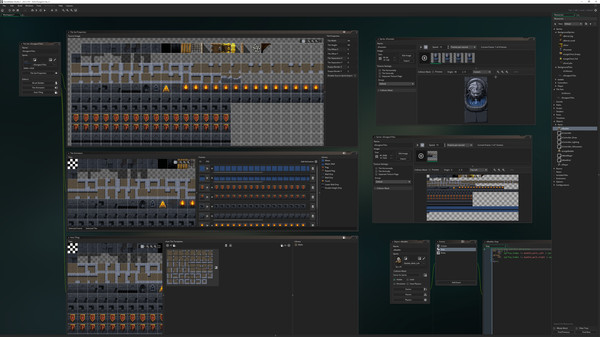
\includegraphics[width=0.8\textwidth]{03.EstudioProblema/01.EstadoArte/00.Figuras/30.interfaz_game_maker.jpg}
    \caption{Interfaz de GameMaker Studio 2. \cite{EA_img_gameMaker}}
    \label{fig:EA_gameMaker}
\end{figure}

Sin embargo, este motor es mucho más limitado que los anteriores en la lista, tanto en capacidad y rendimiento, como en variedad de géneros que puede abarcar, estando limitado a los gráficos 2D o 3D muy básicos. A pesar de estas limitaciones, su versión más reciente (GameMaker Studio 2) permite la distribución en prácticamente todas las plataformas habituales en la actualidad.

GameMaker sigue un modelo de pago anual con posibilidad de realizar una prueba gratuita de 30 días. Una vez terminada la prueba, se deberá adquirir una licencia, que va desde los 39\$ al año para la versión más básica que solo permite publicar en una plataforma: Windows o MacOs. Y los precios aumentan por cada nueva plataforma en la que se quiera publicar: 149\$ para web, 200\$ para Android y iOS, o 799\$ por cada una de las consolas de sobremesa (PS4, Xbox One y Nintendo Switch).

Debido a su facilidad de uso y la no necesidad de conocimientos profundos de informática, es un motor que muchos desarrolladores independientes utilizan para sus juegos. Por ejemplo, para juegos como Crashlands (figura \ref{fig:EA_crashlands}), Hyper Light Drifter o Forager.



\begin{figure}
  \centering
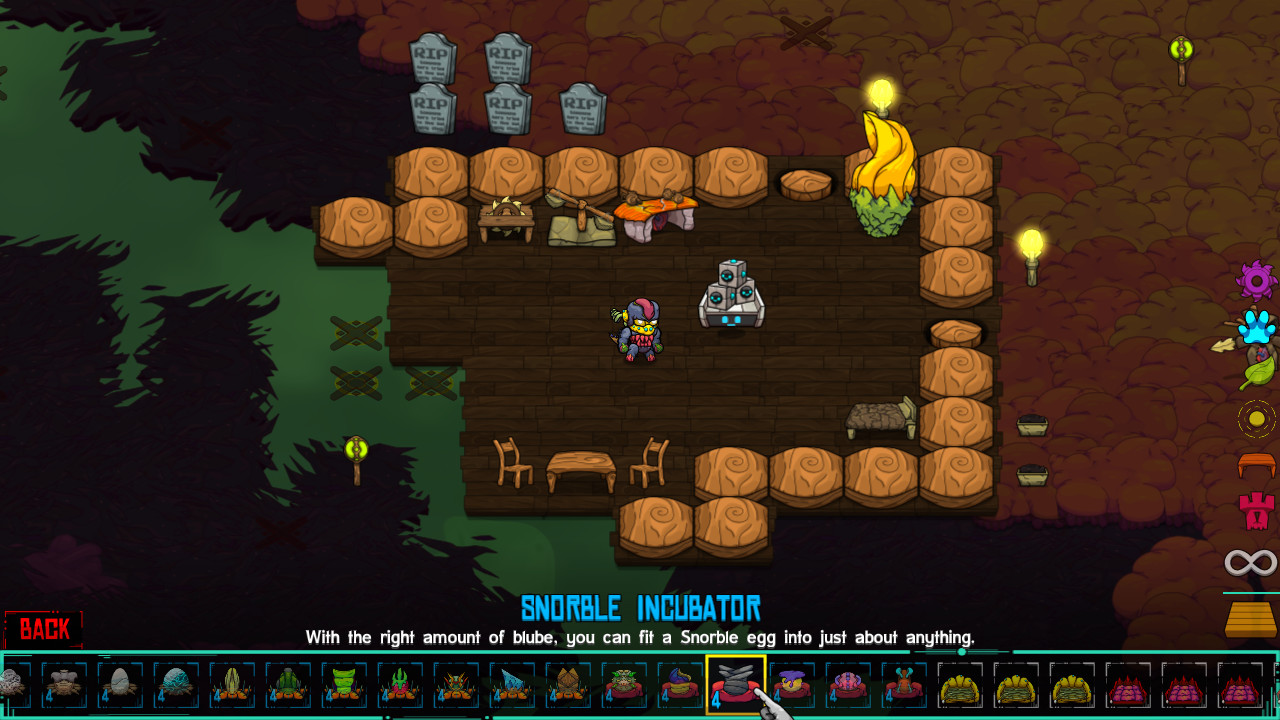
\includegraphics[width=0.8\textwidth]{03.EstudioProblema/01.EstadoArte/00.Figuras/31.crashlands.jpg}
    \caption{Captura de pantalla de Crashlands. \cite{EA_img_crashlands}}
    \label{fig:EA_crashlands}
\end{figure}


\subsection{Godot}

Este motor es el único de la lista que es completamente gratuito y de código abierto. Permite crear todo tipo de videojuegos tanto en 2D como en 3D y además tiene una gran comunidad de desarrolladores en Internet, haciéndolo uno de los motores más fáciles de usar a la vez que versátiles. Figura \ref{fig:EA_godot}.

Godot engine soporta la creación de juegos para PC y dispositivos móviles como Oddventure o RivenTails: Defense (figura \ref{fig:EA_rivenTails}), sin embargo, su soporte para consolas de sobremesa es limitado y no oficial.


\begin{figure}[H]
  \centering
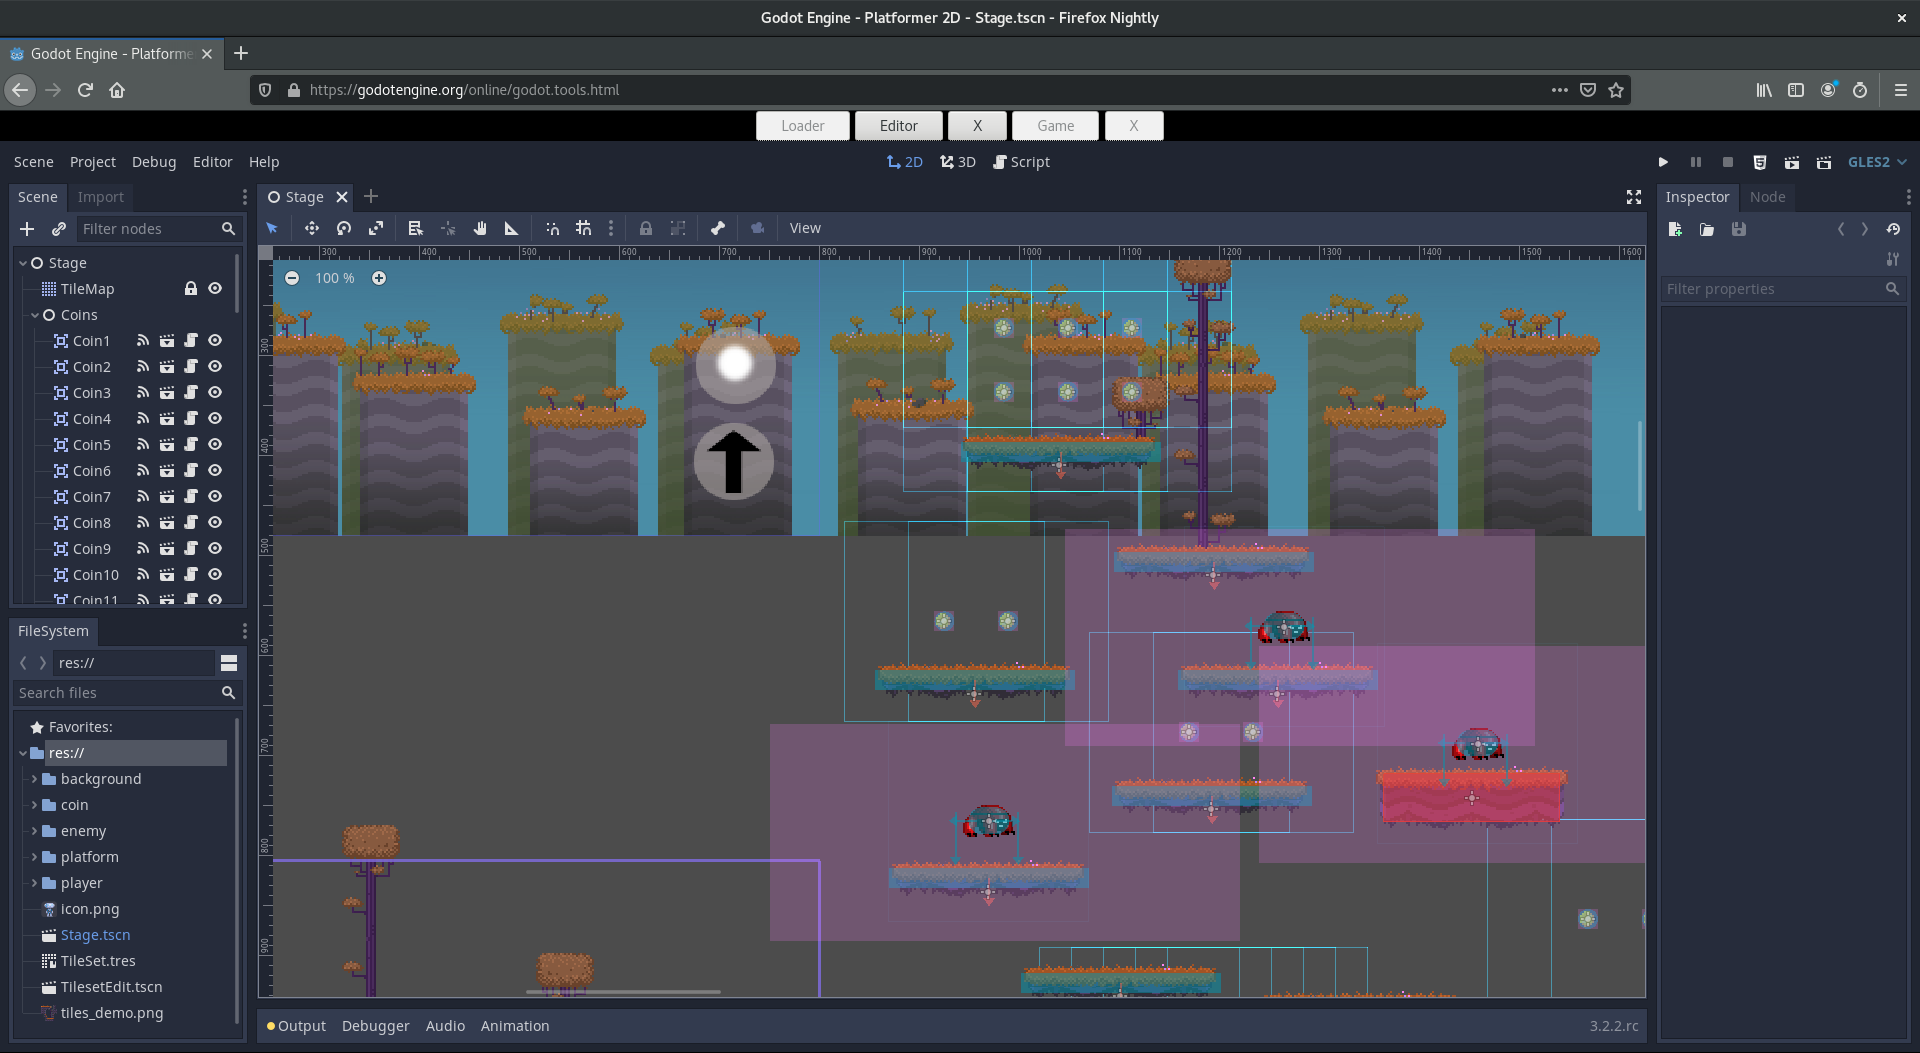
\includegraphics[width=0.8\textwidth]{03.EstudioProblema/01.EstadoArte/00.Figuras/32.interfaz_godot.png}
    \caption{Interfaz de Godot en modo web. \cite{EA_img_godot}}
    \label{fig:EA_godot}
\end{figure}

\begin{figure}[H]
  \centering
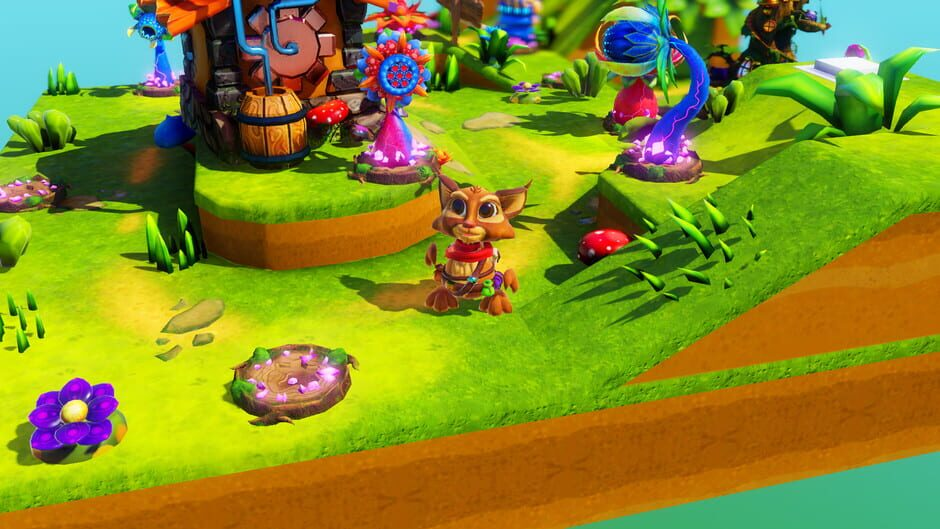
\includegraphics[width=0.8\textwidth]{03.EstudioProblema/01.EstadoArte/00.Figuras/33.riventails_defense.jpg}
    \caption{Captura de pantalla de RivenTails: Defense. \cite{EA_img_rivenTails}}
    \label{fig:EA_rivenTails}
\end{figure}




\section{Conclusión y justificación del proyecto}


La importancia de los ejercicios de brain training para mantener en buen estado las capacidades cognitivas de las personas es evidente, y por ello estos ejercicios han ido evolucionando y cambiando para adaptarse a los distintos medios disponibles. En la actualidad se puede acceder a estos ejercicios desde multitud de dispositivos desde la comodidad del salón. Sin duda esto ha supuesto una mejora en la calidad de vida de muchas personas y de una forma amigable y entretenida, ya que las nuevas tecnologías no solo facilitan el acceso a los ejercicios, si no que los pueden mejorar en gran medida. 

El uso de vídeos, programas interactivos o animaciones coloridas resulta en ejercicios mucho más atractivos para el usuario, que no los verá como una carga o un proceso tedioso, si no como un juego entretenido y divertido. A pesar de esto, los ejercicios actuales tienen raíz en los ejercicios tradicionales y son una evolución directa de los mismos, heredando algunas de sus limitaciones. 

La evolución de la realidad virtual permite que hoy en día puedan crearse experiencias mucho más inmersivas e interactivas que cualquier otra tecnología que utilice una pantalla y métodos de control normales. Aunque en la actualidad existen algunas pruebas utilizando RV aplicada al entrenamiento cognitivo, sigue siendo un campo sin aprovechar completamente.

Es especialmente importante destacar que el entrenamiento cognitivo tiene un componente lúdico que es muy importante aprovechar para mantener al usuario motivado y con ánimo. De igual forma, la realidad virtual no es algo puramente recreativo; puede usarse y se usa con otros propósitos, especialmente en medicina, donde se pueden utilizar modelos 3D de pacientes reales para diagnosticar enfermedades o evaluar intervenciones quirúrgicas incluso antes de realizarlas.

Por este motivo, este proyecto busca complementar la parte lúdica de los ejercicios con el componente serio de la realidad virtual, intentando crear un videojuego que sea capaz de sacar todo el partido a ambos campos.

Por supuesto, esto no sería posible sin la proliferación en popularidad del videojuego, que lo ha convertido en un medio de gran importancia, dando lugar a la creación de motores de videojuegos disponibles para el público, que permiten el desarrollo de videojuegos independientes.



\chapterend
